\documentclass[10pt,a4paper]{article}
\usepackage[margin=21mm,top=20mm,bottom=22mm]{geometry}
\usepackage{newtxtext,newtxmath}
\usepackage{amsmath,mathtools,bm}
\usepackage{graphicx,booktabs,array,float,placeins}
\usepackage[font=small,labelfont=bf,margin=0pt]{caption}
\usepackage{xcolor}
\usepackage[hidelinks]{hyperref}
\usepackage{microtype}
\usepackage{enumitem}
\setlist{nosep,leftmargin=1.4em}
\graphicspath{{figures/}{../pictures/}{../vof/}}
\newcommand{\numHv}{84.5}
\newcommand{\numpsPa}{933}
\newcommand{\numAp}{14.12}
\newcommand{\numQmax}{927}
\newcommand{\numdstar}{0.29}
\newcommand{\numPcHalf}{544}
\newcommand{\numPcOne}{272}
\newcommand{\numPcFour}{68}
\newcommand{\numzlip}{2.71}
\newcommand{\numnSweep}{1127}
\newcommand{\numerrMean}{0.03}
\newcommand{\numerrMax}{1.27}
\newcommand{\numerrMeanS}{0.84}
\newcommand{\numerrMaxS}{9.4}
\newcommand{\numrecQ}{755}
\newcommand{\numrecQfrac}{81}
\newcommand{\numrecN}{36}
\newcommand{\numrecArea}{28.3}
\newcommand{\numrecLam}{1.44}
\newcommand{\numrecTiltLimit}{22.5}
\newcommand{\numrecHmin}{0.5}
\newcommand{\numrecHmax}{2.1}
\newcommand{\numuszZero}{2.2}
\newcommand{\numuszTen}{20.0}
\newcommand{\numuszTwenty}{36.9}
\newcommand{\numuszArea}{468}
\newcommand{\numuszLam}{24}
\newcommand{\numcdh}{0.61}
\newcommand{\nummcRecMed}{1.6}
\newcommand{\nummcRecPnf}{2.2}
\newcommand{\nummcRecFull}{100}
\newcommand{\nummcUszMed}{4.8}
\newcommand{\nummcUszPnf}{24.6}
\newcommand{\nummcUszFull}{0}
\newcommand{\nummcSideMed}{5.6}
\newcommand{\nummcSidePnf}{6.5}
\newcommand{\nummcSideFull}{100}
\newcommand{\nummcCrossMed}{1.6}
\newcommand{\nummcCrossPnf}{2.9}
\newcommand{\nummcCrossFull}{98}
\newcommand{\numnMC}{200}
\newcommand{\numcapFive}{9}
\newcommand{\numcapTen}{12}
\newcommand{\numcapFifteen}{15}
\newcommand{\numcapTwenty}{18}
\newcommand{\numairLo}{19}
\newcommand{\numairHi}{23}

\newcommand{\dd}{\mathrm{d}}
\newcommand{\Lw}{\Lambda_{w}}
\newcommand{\zl}{z_\ell}
\renewcommand{\topfraction}{0.92}
\renewcommand{\textfraction}{0.06}
\renewcommand{\floatpagefraction}{0.8}

\title{\textbf{When does a suction drain stop draining?}\\[3pt]
\large Two-phase hydraulics of a partly submerged perforated drain at $-7$\,mmHg,\\
and a hole layout that keeps it draining}
\author{USZ drain project, technical note\\[2pt]
\small Analysis, simulations and text prepared with Claude Code (Anthropic)}
\date{3 November 2026}

\begin{document}
\maketitle

\begin{abstract}
\noindent
A perforated drain of USZ size (elliptical body $17.85\times9.67$\,mm, 119\,mm long, closed tip, \O4.24\,mm outlet bore centred in the end face) lies in a pool of a glycerol--water mixture and is connected to a regulated suction of $p_s=-7$\,mmHg ($-\numpsPa$\,Pa). As the pool empties, some holes come out of the liquid and suck air. We derive when the drainage stops, test hole layouts and sizes, and confirm the results with two independent simulations.

The air entering the exposed holes and the outlet bore act as two orifices in series. They leave a vacuum $|p_s|/(1+\Lambda^2)$ inside the drain, where $\Lambda$ is the exposed open area divided by the bore area, both weighted by their discharge coefficients. Liquid can leave only through the part of the bore below the inner liquid level, so draining stops when
\[
h + \frac{H_v}{1+\Lambda^2(h)} = \zl, \qquad H_v=\frac{|p_s|}{\rho g}=\numHv\ \text{mm},
\]
where $h$ is the pool level and $\zl$ the height of the bore's lower lip. A refined form accounts for air that must enter against the liquid column inside the drain. Across \numnSweep{} cases (11 layouts, 8 hole sizes from 0.5 to 4\,mm, tilts from $-10^\circ$ to $+20^\circ$), the refined closed form matches a two-phase network simulation with a mean difference of \numerrMean\,mm. A time-dependent simulation reproduces the same stop levels.

The main results are:
\begin{enumerate}[label=(\roman*)]
\item The as-built USZ field ($\numuszArea$\,mm$^2$ open, $\Lambda\approx\numuszLam$) stops at \numuszZero\,mm when lying flat, but at \numuszTen\,mm when the outlet end is $10^\circ$ up and at \numuszTwenty\,mm at $20^\circ$.
\item Hole size matters through the total open area and through how evenly the holes cover the length, not by itself.
\item Two staggered rows at $\pm30^\circ$ from the bottom, $\numrecN\times$\O1.0\,mm (\numrecArea\,mm$^2$, twice the bore area), drain to the lowest hole edge, i.e. a residual level of \numrecHmin--\numrecHmax\,mm, from $-10^\circ$ to $+20^\circ$, and pass \numrecQ\,mL/min while submerged.
\item The intended source is a wall regulator. The recommendation holds as long as the regulator keeps $-7$\,mmHg while passing \numcapTwenty\,L/min of air (\numcapTen\,L/min if the tilt stays within $10^\circ$). A weaker source needs fewer holes; a sizing rule is given.
\end{enumerate}
\end{abstract}

% =============================================================================
\section{The question}
The drain lies in a ``lake'' of liquid with a viscosity between that of water and glycerol. The suction keeps the outlet tube at $-7$\,mmHg. Fluid enters through side holes and leaves through the outlet. The drain is not always level, and as the lake empties, part of the drain sits in air. Two questions follow:
\begin{enumerate}
\item For a given hole layout and hole size, at what pool level does the drain stop removing liquid?
\item Which uniform layout and hole size (0.5 to 4\,mm) keeps it draining longest, so that it leaves the least liquid behind?
\end{enumerate}
``Stops'' means that the liquid flow through the outlet falls below 0.1\,mL/min. Section~\ref{sec:physics} derives the hydraulics and a closed-form stop condition. Section~\ref{sec:layouts} describes the layouts tested. Section~\ref{sec:sim} describes the two simulations used to confirm the analysis, and Section~\ref{sec:results} gives the results. The recommended design is in Section~\ref{sec:design}.

% =============================================================================
\section{Geometry, fluid and operating point}\label{sec:geometry}
We keep the body of the USZ drain from the project package (\texttt{USZ\_drain\_package}) and replace its hole field (Fig.~\ref{fig:geometry}, Table~\ref{tab:params}). The body is an elliptic cylinder lying flat, with outer semi-axes $a=8.925$\,mm (lateral) and $b=4.835$\,mm (vertical), length $L=119$\,mm from the closed tip ($x=0$) to the outlet end face ($x=L$), and a 0.6\,mm skin. The outlet bore (\O4.24\,mm, area $A_p=\numAp$\,mm$^2$) is centred in the end face, roughly half its 9.67\,mm height. The interior is modelled as one open lumen; the fluted inner wall and core of the as-built part are not modelled (Section~\ref{sec:limits}).

A point on the skin is located by its axial position $x$ and by the angle $\theta$ of the parametrisation $y=a\sin\theta$, $z=b(1-\cos\theta)$, with $\theta=0$ the bottom line (6 o'clock), $\pm90^\circ$ the side edges and $180^\circ$ the top. Holes are drilled normal to the skin. The drain may be tilted by $\alpha$ about a horizontal lateral axis; $\alpha>0$ lifts the outlet end. The pool level $h$ is measured from the lowest point of the skin. The lower edge of the bore, the \emph{lip}, then sits at
\begin{equation}
\zl(\alpha) = (b-r_p)\cos\alpha + L\max(\sin\alpha,0), \qquad \zl(0) = \numzlip\ \text{mm},
\label{eq:lip}
\end{equation}
which reaches 23.3\,mm at $\alpha=10^\circ$ and 43.3\,mm at $20^\circ$.

\begin{figure}[!htbp]
\centering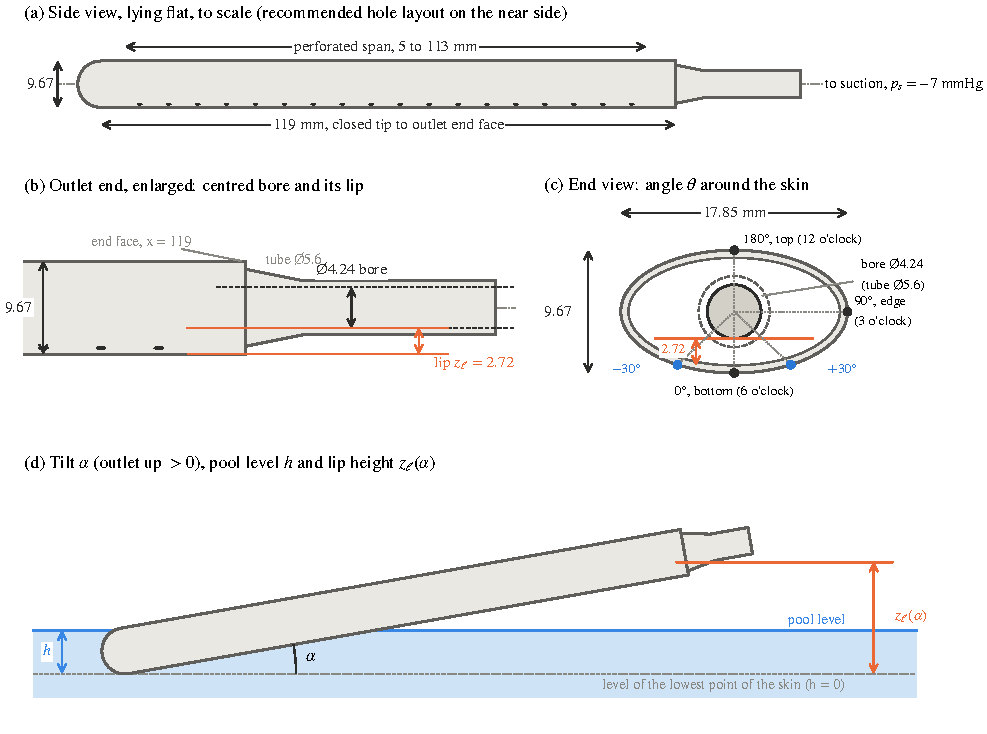
\includegraphics[width=\linewidth]{fig01_geometry.pdf}
\caption{Drain geometry (USZ body). (a) Side view to scale, showing the holes of the recommended layout on the near side. (b) Outlet end: the \O4.24\,mm bore is centred, so its lower lip is $\zl=2.72$\,mm above the bottom of the skin. (c) End view and the angle $\theta$ that locates holes around the skin; the recommended rows sit at $\pm30^\circ$ (blue). (d) Tilt $\alpha$, pool level $h$ and lip height $\zl(\alpha)$, Eq.~\eqref{eq:lip}.}
\label{fig:geometry}
\end{figure}

\begin{table}[!htbp]
\centering\small
\caption{Parameters of the reference case.}\label{tab:params}
\begin{tabular}{@{}l >{\raggedright\arraybackslash}p{0.40\linewidth} >{\raggedright\arraybackslash}p{0.33\linewidth}@{}}
\toprule
quantity & value & note \\
\midrule
outer skin & $17.85\times9.67$\,mm ellipse, $L=119$\,mm & USZ body, lying flat \\
skin thickness $t$ & 0.6\,mm & hole length \\
outlet bore & \O4.24\,mm, $A_p=\numAp$\,mm$^2$, centred & lip at $\zl=\numzlip$\,mm \\
perforated span & $x=5$ to $113$\,mm & as in the USZ part \\
liquid & 50\,wt\% glycerol--water, 20\,$^\circ$C & $\rho=1126$\,kg/m$^3$, $\mu=6.0$\,mPa\,s~\cite{cheng2008}, $\gamma=0.068$\,N/m \\
air & 20\,$^\circ$C & $\rho_a=1.20$\,kg/m$^3$, $\mu_a=1.81\times10^{-5}$\,Pa\,s \\
suction & $p_s=-7$\,mmHg $=-\numpsPa$\,Pa & regulated in the outlet tube \\
suction head & $H_v=|p_s|/\rho g=\numHv$\,mm & Eq.~\eqref{eq:Hv} \\
discharge coefficients & hole $C_h=0.61$ ($d\ge0.8$\,mm) to $0.68$ ($d=0.5$\,mm), bore $C_p=0.85$ & Eqs.~\eqref{eq:cd}, \eqref{eq:cp} \\
pool footprint & $200\times80$\,mm & only for drain times \\
\bottomrule
\end{tabular}
\end{table}

% =============================================================================
\section{Physics}\label{sec:physics}
All pressures are gauge pressures; the atmosphere is $p=0$.

\subsection{Suction head}
At $-7$\,mmHg the suction can hold up a liquid column of
\begin{equation}
H_v=\frac{|p_s|}{\rho g}=\frac{933.3}{1126\times9.81}\ \text{m}=\numHv\ \text{mm}.
\label{eq:Hv}
\end{equation}
This is about nine times the drain height. Gravity and capillarity are therefore not negligible next to the suction, and they decide when the drain stops.

\subsection{Flow through one hole}
A hole of diameter $d$ through a wall of thickness $t$ resists flow through a viscous term and an inertial term in series:
\begin{equation}
\Delta p = R_v\,q + K\,q|q|, \qquad
R_v = \mu\left(\frac{24}{d^3} + \frac{128\,t}{\pi d^4}\right), \qquad
K = \frac{\rho}{2C_h^2A^2}, \qquad A=\frac{\pi d^2}{4}.
\label{eq:hole}
\end{equation}
The first viscous part is Sampson's creeping flow through a circular aperture in a thin plate~\cite{sampson1891}. The second is Hagen--Poiseuille flow along the bore. Their sum approximates the exact finite-length solution well~\cite{dagan1982}. The inertial part is the orifice law with discharge coefficient $C_h$, which depends on $t/d$~\cite{lichtarowicz1965}:
\begin{equation}
C_h = 0.61 \ \ (t/d\le0.75), \qquad C_h \text{ rising linearly to } 0.81 \ \ (t/d\ge2).
\label{eq:cd}
\end{equation}
For $t=0.6$\,mm this gives $C_h=0.61$ for $d\ge0.8$\,mm. Solving Eq.~\eqref{eq:hole} for $q$ gives the numerically stable form
\begin{equation}
q=\frac{2\,\Delta p}{R_v+\sqrt{R_v^2+4K\Delta p}}.
\label{eq:hole-q}
\end{equation}
For the liquid at $\Delta p\approx0.5$\,kPa and $d=1$\,mm the hole Reynolds number is about 100, and the viscous term lowers the flow by about 12\,\% relative to the pure orifice law; at $d=0.5$\,mm it lowers it by about 40\,\%. For air, $\mu_a/\mu=0.003$ and the viscous term is negligible. A hole that is partly submerged is split by area into a submerged fraction $f_s$ and an exposed fraction $f_e$, each treated as a hole of area $fA$ (that is, $R_v/f$ and $K/f^2$).

\subsection{Why an exposed hole leaks air}
When the liquid surface drops below a hole, a meniscus forms in it. It can resist the suction behind it only up to the capillary entry pressure
\begin{equation}
P_c=\frac{4\gamma\cos\theta_e}{d}\le\frac{4\gamma}{d},
\label{eq:pc}
\end{equation}
where $\theta_e$ is the effective contact angle (with edge pinning the maximum is $4\gamma/d$~\cite{oliver1977,degennes2004}). The largest possible value is \numPcHalf\,Pa for $d=0.5$\,mm, \numPcOne\,Pa for $d=1$\,mm and \numPcFour\,Pa for $d=4$\,mm. All of these are below $|p_s|=\numpsPa$\,Pa. A hole seals against the full suction only if
\begin{equation}
d < d^* = \frac{4\gamma}{|p_s|} = \numdstar\ \text{mm},
\label{eq:dstar}
\end{equation}
even with perfect wetting. Every hole in the 0.5 to 4\,mm range therefore lets air in as soon as it is exposed. Once air passes, the hole stays open until it is submerged again. Capillarity plays a role only after the vacuum inside the drain has already dropped, and it is treated as a sensitivity case ($\theta_e=60^\circ$ and $0^\circ$; the baseline is $\theta_e=90^\circ$, no holding).

\subsection{The outlet bore}
The flow contracts from the drain lumen ($\approx110$\,mm$^2$) into the bore ($14.1$\,mm$^2$), an area ratio $\sigma\approx0.13$. Weisbach's contraction coefficient $C_c=0.63+0.37\sigma^3\approx0.63$ gives a loss coefficient $K_c=(1/C_c-1)^2\approx0.35$~\cite{idelchik1994}. Because $p_s$ is the static pressure in the outlet tube, the bore behaves as an orifice with
\begin{equation}
C_p = (1+K_c)^{-1/2}\approx0.85, \qquad
Q_{max}=C_pA_p\sqrt{\frac{2|p_s|}{\rho}}=\numQmax\ \text{mL/min}.
\label{eq:cp}
\end{equation}
$Q_{max}$ is the most liquid that the bore can pass at $-7$\,mmHg. As Section~\ref{sec:results} shows, the bore, not the holes, is the main restriction whenever the open hole area exceeds about twice the bore area.

\subsection{The flow network at one pool level}\label{sec:network}
Inside the drain there is a gas pressure $p_g$ and a horizontal inner liquid level $\zeta$; the drain is full of liquid when $\zeta$ lies above its top. The pressure on the inner side of a hole at height $z$ is
\begin{equation}
p_{in}(z)=p_g+\rho g\,(\zeta-z)^+ ,
\end{equation}
where $(\cdot)^+$ means $\max(\cdot,0)$. For opening $j$, with submerged and exposed parts at mean heights $z^s_j$ and $z^e_j$, the network has the following flows:
\begin{align}
\text{liquid in:}\quad & \Delta p^L_j = \rho g\,(h-z^s_j) - p_{in}(z^s_j), \label{eq:liqin}\\
\text{air in:}\quad & \Delta p^G_j = -p_{in}(z^e_j) \ \ \text{if the opening is open to air},\label{eq:gasin}\\
\text{liquid out of an exposed hole:}\quad & \Delta p = p_{in}(z^e_j)>0 \ \ \text{if its inner side is wet.}\label{eq:leak}
\end{align}
Each flow follows Eq.~\eqref{eq:hole-q}. An exposed opening becomes open to air when $-p_{in}(z^e_j)>P_c$. At the bore, gravity separates the phases (a separated-flow model~\cite{wallis1969}): liquid leaves through the part of the bore below $\zeta$ and gas through the part above it,
\begin{equation}
A_L = A_p\,F\!\left(\frac{\zeta-z_c}{r_p\cos\alpha}\right),\quad
F(u)=\frac{\pi-\arccos u+u\sqrt{1-u^2}}{\pi},\qquad A_G=A_p-A_L,
\end{equation}
\begin{equation}
q_{L,b}=C_pA_L\sqrt{\frac{2\,(p_g-p_s+\rho g\,(\zeta-\bar z_L))}{\rho}},\qquad
q_{G,b}=C_pA_G\sqrt{\frac{2\,(p_g-p_s)}{\rho_a}},
\label{eq:bore}
\end{equation}
where $z_c$ is the bore centre and $\bar z_L$ the centroid of the liquid part. The two unknowns $(p_g,\zeta)$ follow from conservation of liquid and gas:
\begin{equation}
\sum_j q^L_j-\sum_j q^{leak}_j=q_{L,b},\qquad \sum_j q^G_j = q_{G,b}.
\label{eq:balance}
\end{equation}

\begin{figure}[!htbp]
\centering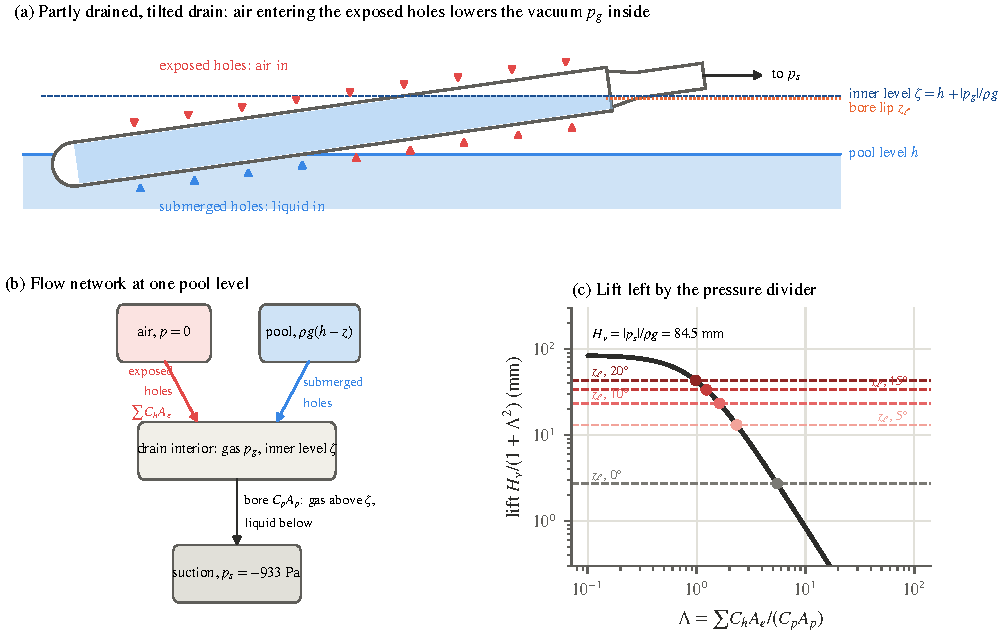
\includegraphics[width=\linewidth]{fig02_mechanism.pdf}
\caption{Mechanism. (a) Once holes are exposed, air enters through them while liquid still enters through the submerged ones. The liquid inside the drain stands at $\zeta=h+|p_g|/\rho g$ and can leave only through the part of the bore below $\zeta$. (b) The flow network solved at each pool level, Eqs.~\eqref{eq:liqin}--\eqref{eq:balance}. (c) The vacuum left inside the drain, expressed as a liquid lift, against the exposed-area ratio $\Lambda$. The dashed lines are the lip heights $\zl(\alpha)$, and the dots mark the largest $\Lambda$ that still lifts the liquid to the lip.}
\label{fig:mechanism}
\end{figure}

\subsection{The pressure divider}
Neglect the liquid column inside the drain and the viscous gas terms. The gas balance in Eq.~\eqref{eq:balance} then involves two orifices in series, the exposed holes and the bore:
\[
\sum_j C_{h,j}A^e_j\sqrt{\frac{2(-p_g)}{\rho_a}} = C_pA_p\sqrt{\frac{2(p_g-p_s)}{\rho_a}}
\quad\Longrightarrow\quad
-p_g = \frac{|p_s|}{1+\Lambda^2},\qquad
\Lambda=\frac{\sum_j C_{h,j}A^e_j}{C_pA_p}.
\]
The gas density and the size of the air flow both drop out, so the vacuum left inside depends only on the area ratio $\Lambda$. With $\Lambda=1$, half the suction remains. The as-built USZ field reaches $\Lambda\approx12$ as soon as its top face is exposed, which leaves 0.7\,\% of the suction, or 0.6\,mm of lift.

\subsection{Lift, and the stop condition}
Liquid can leave only if the inner level reaches the bore lip, $\zeta\ge\zl$. When no liquid flows, the pressure balance across a submerged hole is $\rho g(h-z)=p_g+\rho g(\zeta-z)$, so the vacuum lifts the inner liquid to
\begin{equation}
\zeta = h + \frac{|p_g|}{\rho g}.
\end{equation}
Drainage is therefore possible only while $h+|p_g|/\rho g>\zl$. Combined with the pressure divider, the drain stops at the level $h_s$ that satisfies
\begin{equation}
h_s + \frac{H_v}{1+\Lambda(h_s)^2} = \zl \qquad\text{(simple bound).}
\label{eq:stop-simple}
\end{equation}
This bound treats every exposed hole as if air entered it at the full inner vacuum. An exposed hole that lies \emph{below} the inner level ($z<\zeta$) admits air only by pushing against the liquid column $\rho g(\zeta-z)$. At the threshold, where $\zeta=\zl$ and $-p_g=\rho g(\zl-h)$, the air entering an exposed element at height $z$ is driven by $\rho g(\min(z,\zl)-h)$ instead of $\rho g(\zl-h)$. Weighting each exposed element by $w=(\min(z,\zl)-h)/(\zl-h)$ gives the refined stop condition
\begin{equation}
\boxed{\;h_s + \frac{H_v}{1+\Lw(h_s)^2} = \zl,\qquad
\Lw(h)=\frac{1}{C_pA_p}\sum_{\text{exposed}} C_h\,\delta A\,\sqrt{w}\;}
\qquad\Lw\le\Lambda.
\label{eq:stop-refined}
\end{equation}
The left side increases with $h$, because $\Lw$ never increases as $h$ rises, so the root is unique. Drainage also needs liquid that can reach a hole, so it stops at the latest when the pool falls below the lowest edge of the lowest hole, $h_{geo}$. Overall, $h_s=\max(h_{geo},\ \text{root of Eq.~\eqref{eq:stop-refined}})$. Three consequences follow:
\begin{enumerate}
\item While $h>\zl$, no lift is needed: liquid reaches the bore whatever the vacuum, so the drain keeps draining. Every drain therefore empties the pool at least down to the lip, $h_s<\zl$, which is 2.7\,mm for a drain lying flat.
\item With the outlet up, the lip rises by $L\sin\alpha$, and the vacuum has to lift the liquid much further.
\item The drain empties the pool down to its lowest hole only if
\begin{equation}
\Lw(h_{geo}) < \Lambda^* = \sqrt{\frac{H_v}{\zl(\alpha)-h_{geo}}-1}.
\label{eq:lstar}
\end{equation}
Taking $h_{geo}=0$ gives $\Lambda^*=5.5$ at $0^\circ$, $2.3$ at $5^\circ$, $1.6$ at $10^\circ$ and $1.0$ at $20^\circ$. Beyond $\alpha\approx44^\circ$ the lip is higher than $H_v$, and no layout can empty the pool below $\zl-H_v$.
\end{enumerate}

\subsection{A suction source with limited capacity}
A real pump or regulator holds $p_s$ only up to some volume flow $Q_s$. Once the air drawn through the exposed holes exceeds $Q_s$, the source is saturated, and the vacuum inside follows from the holes alone, $|p_g|\approx(\rho_a/2)\,(Q_s/\sum C_hA^e)^2$. Full drainage then additionally requires
\begin{equation}
\sum C_hA^e \ <\ \frac{Q_s}{\sqrt{2\rho g\,(\zl-h_{geo})/\rho_a}}.
\label{eq:cap-area}
\end{equation}
For example, at $\alpha=10^\circ$ a 5\,L/min source can feed only about 7\,mm$^2$ of exposed hole area at the vacuum that the lift requires.

\subsection{Draining in time}
The pool level falls as $\dd h/\dd t=-Q_L(h)/A_{fs}(h)$, where $Q_L$ is the net liquid inflow to the drain and $A_{fs}$ is the pool's free-surface area (pool footprint minus the drain's footprint at that level). Because the drain interior settles within seconds, much faster than the pool, $Q_L(h)$ can be taken from the steady network at each level (Section~\ref{sec:sim}). Air entrainment by surface drawdown above an active hole (critical submergence~\cite{gordon1970}) is included as a sensitivity case: a hole is counted as exposed once the surface is within $\kappa d$ of it, with $\kappa=0.5$.

% =============================================================================
\section{Hole distributions tested}\label{sec:layouts}
Ten uniform layouts (A to J) plus the as-built USZ field were tested (Figs.~\ref{fig:patterns}, \ref{fig:3d}). In every layout the holes are equally spaced along $x$ within each row. The layouts differ in the number of rows, their angles $\theta$ and their axial alignment (in line, staggered by half a pitch, or helical):

\noindent
A side rows (3 and 9 o'clock); B top and bottom; C four rows in line; D helix over the same four positions; E eight rows evenly around the skin; F both faces at $\pm45^\circ$ and $\pm135^\circ$; G lower band ($0^\circ$, $\pm45^\circ$); H lower flanks $\pm45^\circ$ in line; I the same staggered; J one bottom row. The recommended layout (two staggered rows at $\pm30^\circ$) came out of the optimisation in Section~\ref{sec:opt}.

Each layout was built with eight hole diameters, $d=0.5$ to $4.0$\,mm in 0.5\,mm steps, in two families (Fig.~\ref{fig:sizes}):
\begin{description}[leftmargin=1em]
\item[Fixed count:] 19 holes per row (pitch 5.7\,mm), so the open area grows as $d^2$.
\item[Fixed area:] the number of holes is chosen so that the total open area is about $2A_p=28$\,mm$^2$, so larger holes mean fewer holes.
\end{description}
Tilts of $-10^\circ$ to $+20^\circ$ in $5^\circ$ steps give $\numnSweep$ cases.

\begin{figure}[p]
\centering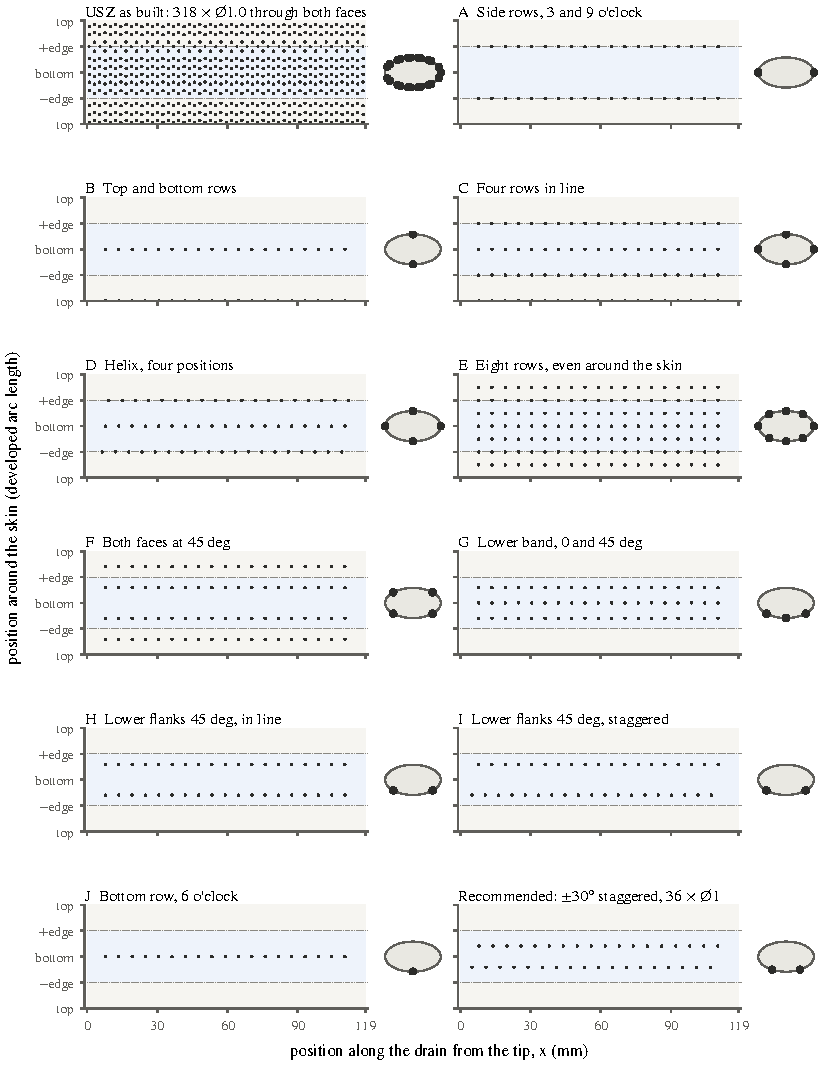
\includegraphics[width=\linewidth]{fig03_patterns.pdf}
\caption{All tested hole distributions, drawn on the unrolled skin (to scale, \O1.0\,mm, 19 holes per row). The horizontal axis is the position along the drain; the vertical axis runs once around the skin (bottom in the middle, side edges dotted, top at both edges). The small end views show where the rows sit. Dark holes on the light-blue band face downward when the drain lies flat. The recommended layout (last panel) has two rows at $\pm30^\circ$, staggered by half a pitch.}
\label{fig:patterns}
\end{figure}

\begin{figure}[!htbp]
\centering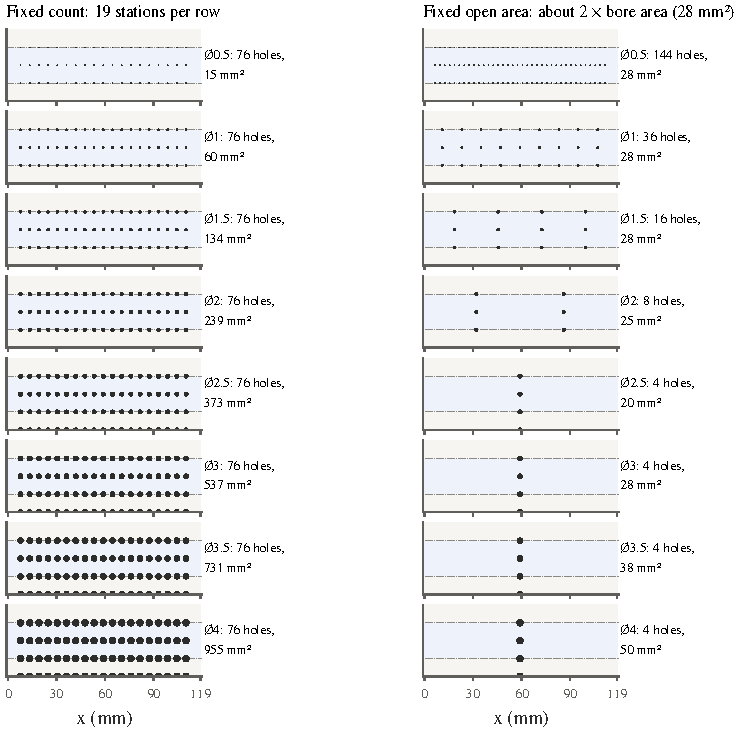
\includegraphics[width=\linewidth]{fig04_sizes.pdf}
\caption{Hole-size families, shown for layout C. Left: fixed count, so the open area grows from 15 to 955\,mm$^2$. Right: fixed open area of about 28\,mm$^2$. Large holes then come in very few stations; from 2.5\,mm on, all holes sit at mid-length, which leaves the ends of the drain without holes.}
\label{fig:sizes}
\end{figure}

\begin{figure}[!htbp]
\centering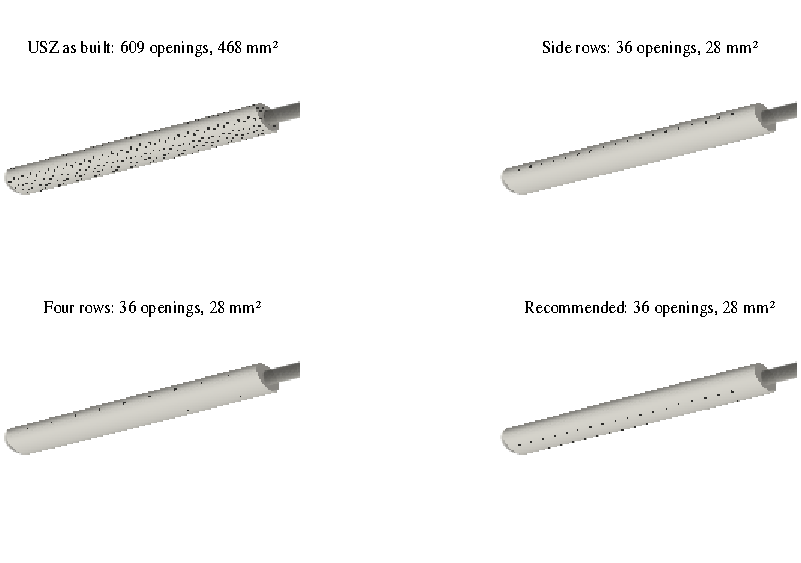
\includegraphics[width=0.94\linewidth]{fig05_3d.pdf}
\caption{3D views (from below and in front, outlet tube on the right) of the as-built USZ field, side rows, four rows and the recommended layout.}
\label{fig:3d}
\end{figure}

% =============================================================================
\section{Simulations used to confirm the analysis}\label{sec:sim}
The closed form was checked against two numerical models that drop its simplifications. A three-dimensional two-phase CFD check (volume of fluid) is set up as well (Section~\ref{sec:cfd}), but its results are not yet available.

\paragraph{Quasi-static two-phase network.} Each opening is split into 61 equal-area elements (a Vogel spiral on the developed skin), mapped to their true height for the tilt. At each pool level the solver finds the submerged and exposed fractions of every opening and solves Eqs.~\eqref{eq:liqin}--\eqref{eq:balance}. It includes:
\begin{itemize}
\item viscous and inertial losses in every opening;
\item hydrostatics inside the drain, and liquid dripping out of exposed holes;
\item gas and liquid sharing the bore;
\item the capillary breakthrough state of each opening, which persists until the opening is submerged again;
\item optionally, a source with limited capacity.
\end{itemize}
The two unknowns are found by nested monotone root finding (Illinois false position): $p_g$ from the gas balance for a given $\zeta$, and $\zeta$ from the liquid balance. If the liquid balance is negative even with $\zeta$ at the lip, the drain is stalled. The pool is lowered in 0.1\,mm steps, and the stop level is then refined by bisection to 0.01\,mm. Drain times come from integrating $\dd t=A_{fs}\,\dd h/Q_L$.

\paragraph{Time-dependent simulation.} This model does not assume a steady interior. The liquid stored inside the drain, $V_L$, is a state variable:
\begin{equation}
\frac{\dd V_L}{\dd t}=Q_{L,in}-Q_{leak}-q_{L,b},\qquad
\frac{\dd h}{\dd t}=-\frac{Q_{L,in}-Q_{leak}}{A_{fs}},\qquad
0=Q_{L,in}+Q_{G,in}-Q_{leak}-q_{L,b}-q_{G,b}.
\end{equation}
The last equation states that the rigid drain conserves volume, and it fixes $p_g$ at every instant (gas compressibility acts on microsecond scales at 1\,\% pressure changes). The inner level $\zeta$ follows from $V_L$ through the interior geometry. $V_L$ is advanced with backward Euler, which is stable for the stiff bore, and $h$ explicitly with steps of at most 0.05\,mm. Openings break through and reseal as in the network model. The run ends once no liquid has left the drain for two minutes.

\paragraph{Agreement.} Over all \numnSweep{} sweep cases, the refined closed form, Eq.~\eqref{eq:stop-refined}, matches the network simulation with a mean absolute difference of \numerrMean\,mm and a maximum of \numerrMax\,mm (Fig.~\ref{fig:parity}). The simple bound, Eq.~\eqref{eq:stop-simple}, is conservative: it overestimates the stop level by up to \numerrMaxS\,mm at outlet-up tilts. The time-dependent simulation ends at the same levels to within 0.02\,mm (Table~\ref{tab:validation}); Fig.~\ref{fig:transient} shows its time histories.

\begin{figure}[!htbp]
\centering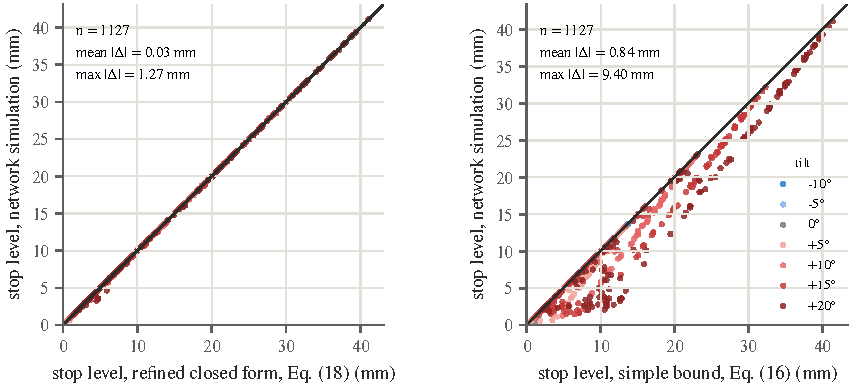
\includegraphics[width=\linewidth]{fig11_parity.pdf}
\caption{Stop level from the network simulation against the closed forms, for all \numnSweep{} cases (colour gives the tilt). Left: refined condition, Eq.~\eqref{eq:stop-refined}. Right: simple bound, Eq.~\eqref{eq:stop-simple}, which is conservative when air must enter against liquid standing inside a tilted drain.}
\label{fig:parity}
\end{figure}

\begin{table}[!htbp]
\centering\small
\caption{Stop level $h_s$ (mm above the lowest point of the skin) from the three methods, for four designs. ``Four rows'' and ``side rows'' are the fixed-area (28\,mm$^2$) versions.}\label{tab:validation}
\begin{tabular}{@{}l r r r r r@{}}
\toprule
design & $\alpha$ & closed form & network & time-dependent & lowest hole edge \\
 & & Eq.~\eqref{eq:stop-refined} & (quasi-static) & simulation & $h_{geo}$ \\
\midrule
Recommended & $0^\circ$ & 0.51 & 0.52 & 0.51 & 0.53 \\
Recommended & $10^\circ$ & 1.35 & 1.36 & 1.36 & 1.37 \\
USZ as built & $0^\circ$ & 2.29 & 2.21 & 2.21 & 0.01 \\
USZ as built & $10^\circ$ & 20.13 & 19.97 & 19.97 & 0.11 \\
Side rows & $0^\circ$ & 4.35 & 4.37 & 4.36 & 4.37 \\
Side rows & $10^\circ$ & 5.67 & 5.67 & 5.67 & 5.69 \\
Four rows & $0^\circ$ & 0.00 & 0.00 & 0.00 & 0.01 \\
Four rows & $10^\circ$ & 1.81 & 1.83 & 1.82 & 1.83 \\
\bottomrule
\end{tabular}

\end{table}

\begin{figure}[!htbp]
\centering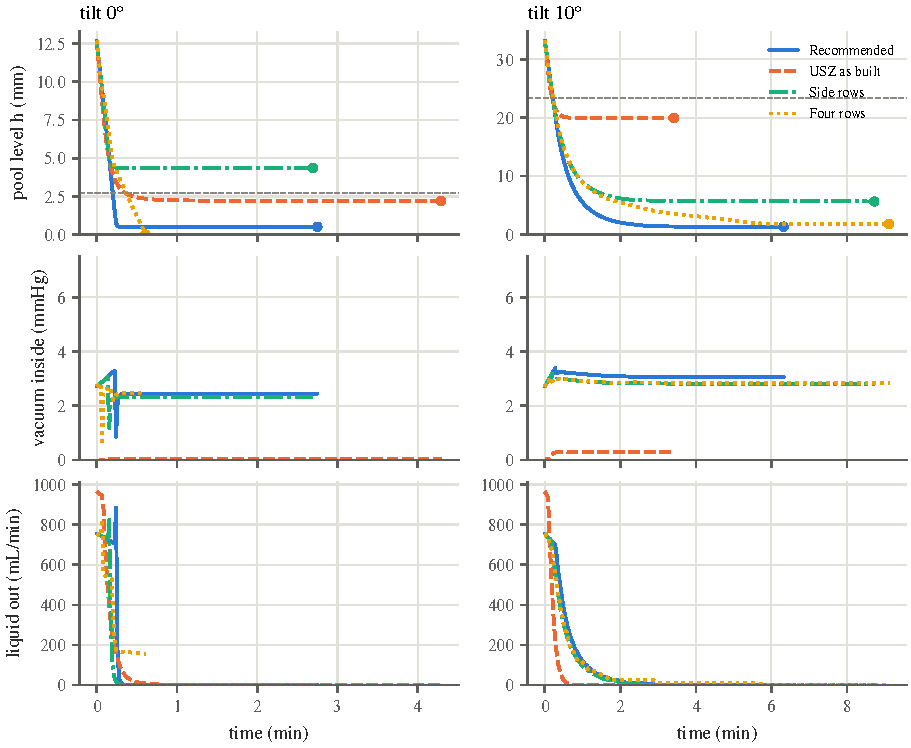
\includegraphics[width=\linewidth]{fig13_transient.pdf}
\caption{Time-dependent simulation (pool $200\times80$\,mm, starting 3\,mm above the drain): pool level, vacuum inside the drain and liquid leaving through the bore. The dots mark where the drainage has stopped.}
\label{fig:transient}
\end{figure}

% =============================================================================
\section{Results}\label{sec:results}

\subsection{How the drainage stops}
Figure~\ref{fig:curves} follows five designs as the pool falls. While all holes are submerged, the drains pass 720 to 970\,mL/min, close to the bore limit $Q_{max}=\numQmax$\,mL/min. The vacuum at the bore end of the interior is only about 2.4\,mmHg; the bore itself takes the rest of the 7\,mmHg. With the large USZ field, the interior even sits slightly above atmospheric pressure, because all the suction acts across the bore.

As soon as the upper holes of the USZ field are exposed, the interior vacuum collapses ($\Lambda\gg1$). The drain then keeps emptying only while the pool is above the lip, which is 2.7\,mm when flat and 23.3\,mm at $10^\circ$, and it stops just below. A layout with little open area keeps 2 to 3\,mmHg inside and drains on until its lowest holes are uncovered. Side rows stop at about mid-height (4.4\,mm when flat): this is a geometric stop, because nothing lower can take in liquid.

Figure~\ref{fig:pictures} draws the state that the network simulation computes, for both designs at $10^\circ$, with every opening coloured by what flows through it.
\begin{itemize}
\item \textbf{USZ at its stop (29\,s).} About 28\,L/min of air pours in through the exposed openings, and the vacuum inside falls to 37\,Pa. That vacuum still holds the liquid in the drain 3.4\,mm above the pool, but only up to the bore lip, so the submerged openings stop flowing.
\item \textbf{Recommended layout at the same moment.} It keeps $-$432\,Pa inside and drains 397\,mL/min, with air entering only through the few exposed openings near the outlet.
\item \textbf{Recommended layout at the end (153\,s).} It stops when its lowest openings leave the pool, at 1.4\,mm.
\end{itemize}
An animation of the whole drainage is in \texttt{pictures/drain\_emptying\_tilt10.gif}.

\begin{figure}[!htbp]
\centering
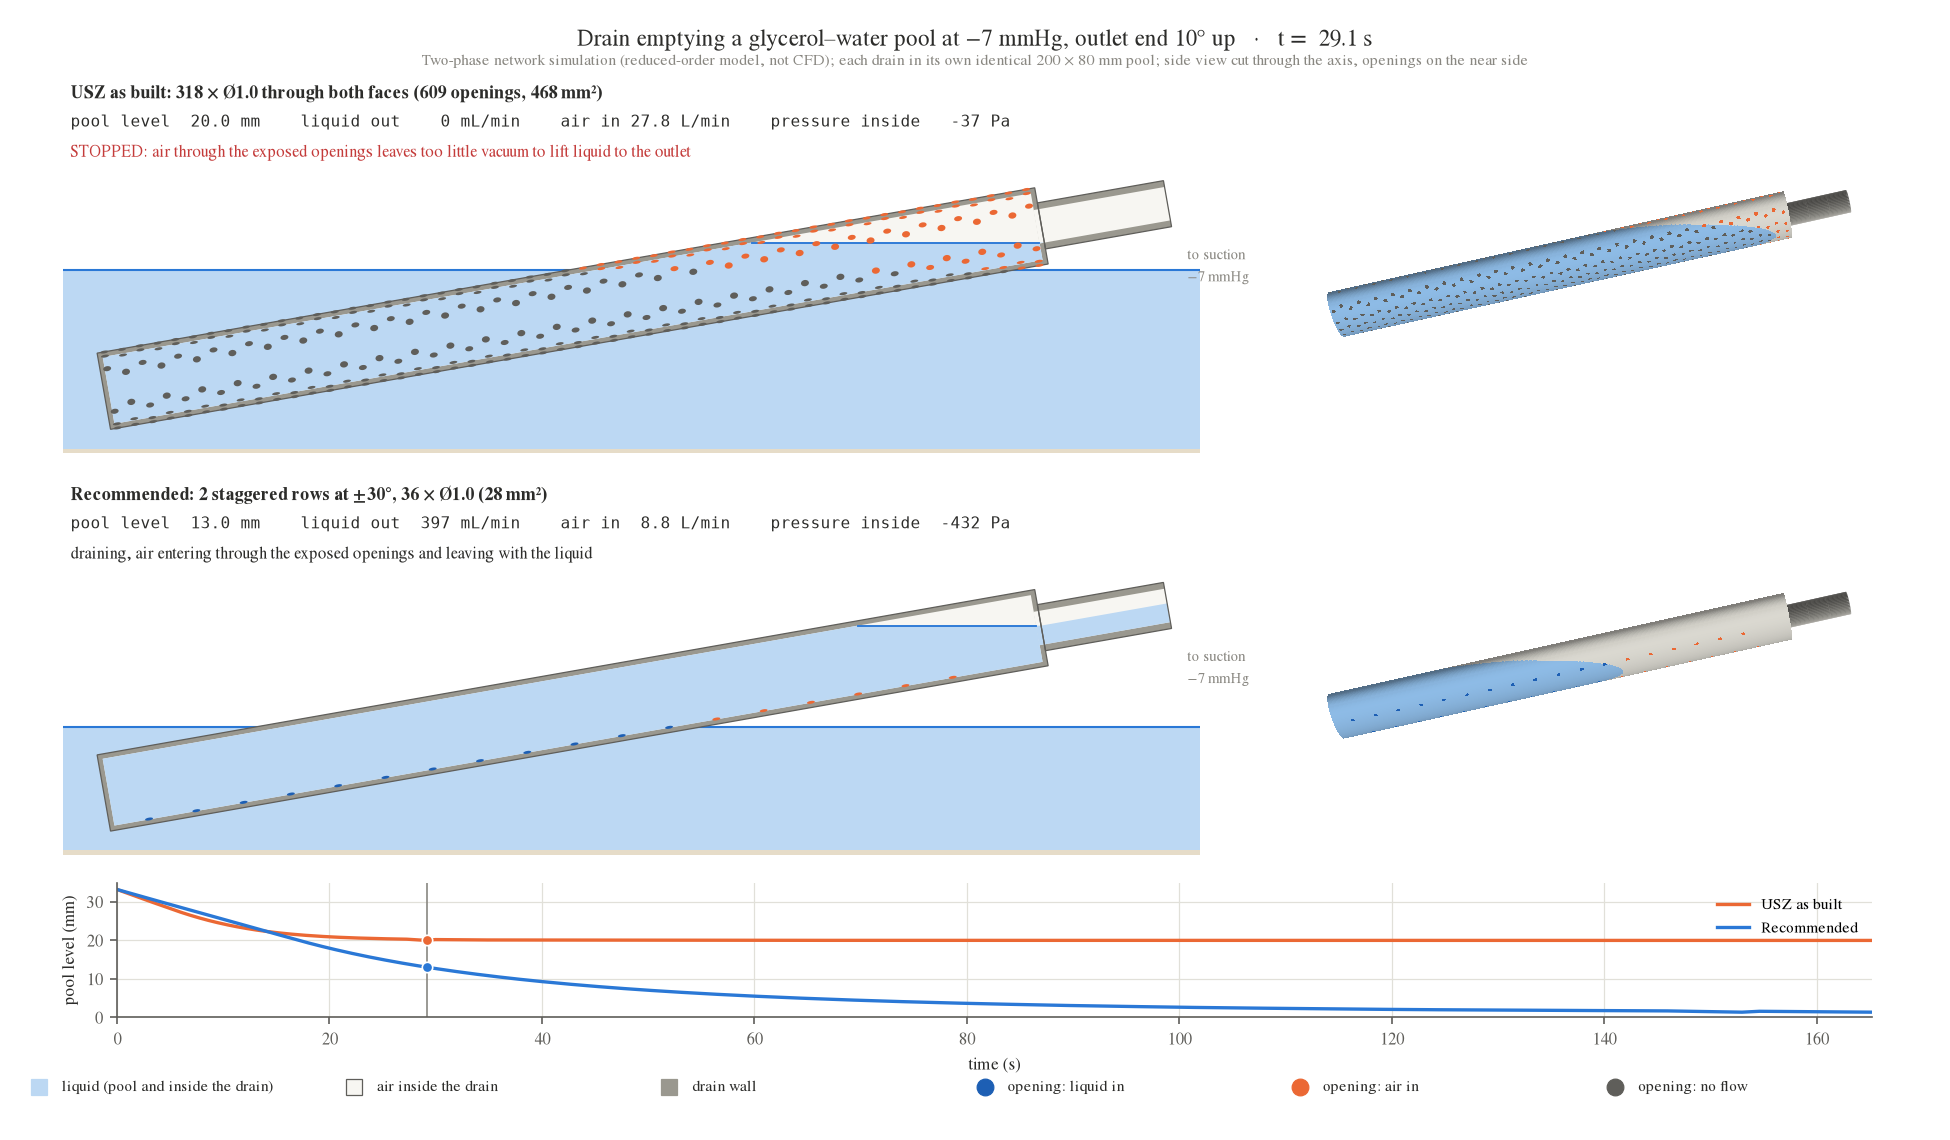
\includegraphics[width=\linewidth]{tilt10_3_usz_stops.png}\\[2mm]
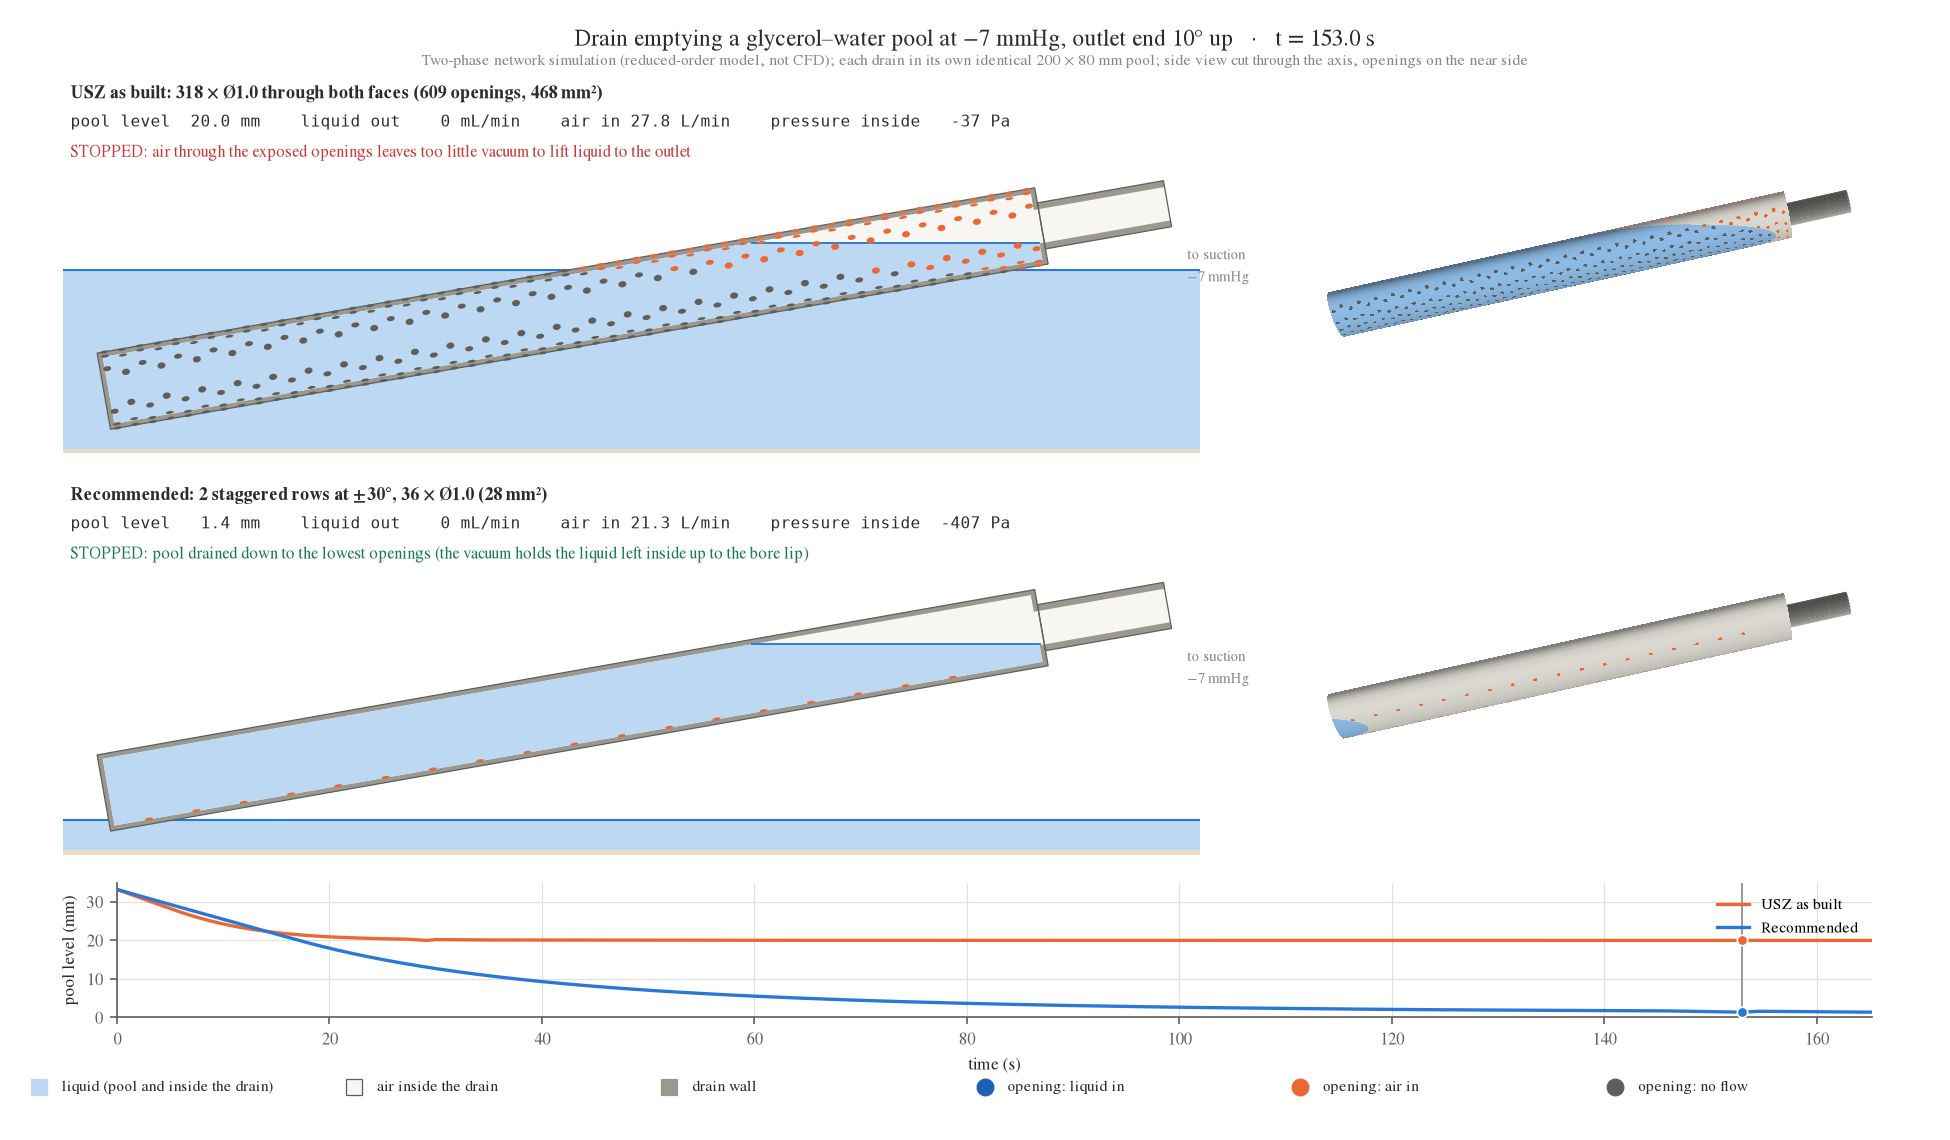
\includegraphics[width=\linewidth]{tilt10_4_end.png}
\caption{State of the network simulation while the pool empties, outlet end $10^\circ$ up, each drain in its own identical pool. Top: the moment the USZ part stops (20.0\,mm). Bottom: the recommended part has drained to its lowest openings (1.4\,mm). Each panel shows three views. Left: a cut through the drain axis with the pool, the liquid and air inside the drain, and the near-side openings, coloured blue for liquid in, orange for air in and grey for no flow. Right: a 3D view from below. Bottom: the pool level against time. These are states of the reduced-order model, not CFD fields.}
\label{fig:pictures}
\end{figure}

\begin{figure}[!htbp]
\centering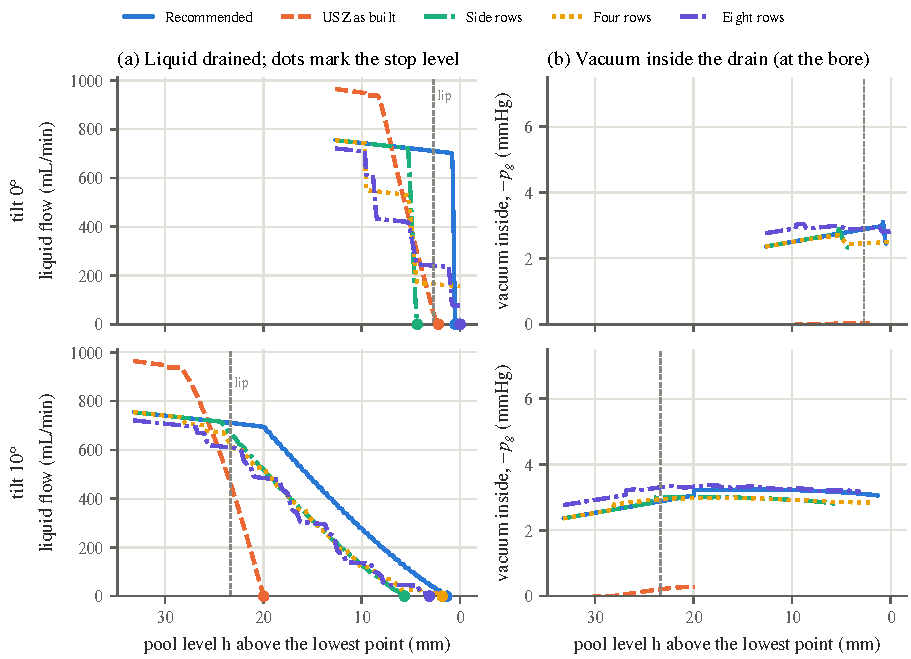
\includegraphics[width=\linewidth]{fig07_drainage_curves.pdf}
\caption{Quasi-static drainage of five designs, read from right to left as the pool falls. (a) Liquid drained; the dots mark the stop level. (b) Vacuum inside the drain at the bore. The dashed line is the lip height $\zl(\alpha)$. Top row: flat; bottom row: outlet $10^\circ$ up.}
\label{fig:curves}
\end{figure}

\subsection{Effect of layout, hole size and tilt}
Table~\ref{tab:layouts} and Figs.~\ref{fig:hcount}--\ref{fig:heat} give the stop level of every case. The main findings:
\begin{itemize}
\item \textbf{The as-built USZ field} drains well only when flat, stopping at \numuszZero\,mm just below the lip. Any outlet-up tilt leaves a deep pool (\numuszTen\,mm at $10^\circ$), because its 468\,mm$^2$ of openings give $\Lambda\approx24$.
\item \textbf{Total open area is the main design variable.} With a fixed count (open area $\propto d^2$), the layouts that tolerate tilt with small holes fail with the outlet up once $d$ exceeds about 1 to 2\,mm, when the open area passes roughly 60 to 130\,mm$^2$ (Fig.~\ref{fig:hcount}). With a fixed area of 28\,mm$^2$, every layout stops below about 7\,mm at all tilts, and the side rows are the worst when flat (Table~\ref{tab:layouts}).
\item \textbf{Placement around the skin} sets the geometric limit. Holes at mid-height or above (A, and the upper parts of E and F) cannot remove the last millimetres, while holes on the lower half can.
\item \textbf{Placement along the length} matters under tilt. The lowest point is the tip when the outlet is up and the outlet end when it is down, so holes must reach both ends. With a fixed area, large holes come in so few stations that the ends stay uncovered (Fig.~\ref{fig:harea}, Table~\ref{tab:sizes}). Staggering two rows halves the effective axial pitch, which is why layout I beats H at positive tilt.
\end{itemize}

\begin{figure}[!htbp]
\centering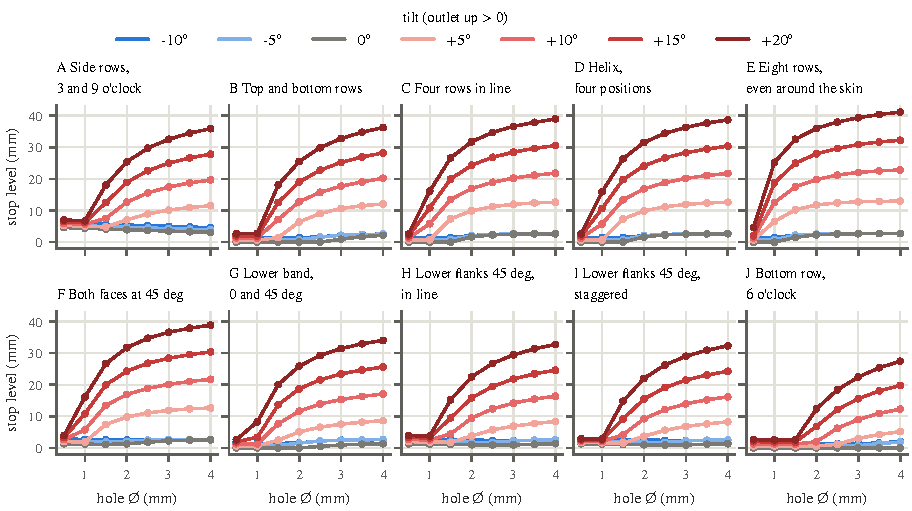
\includegraphics[width=\linewidth]{fig08_hstop_vs_d_count.pdf}
\caption{Stop level against hole diameter, fixed-count family (19 holes per row). Colour gives the tilt: blue for outlet down, grey for flat, red for outlet up.}
\label{fig:hcount}
\end{figure}

\begin{figure}[!htbp]
\centering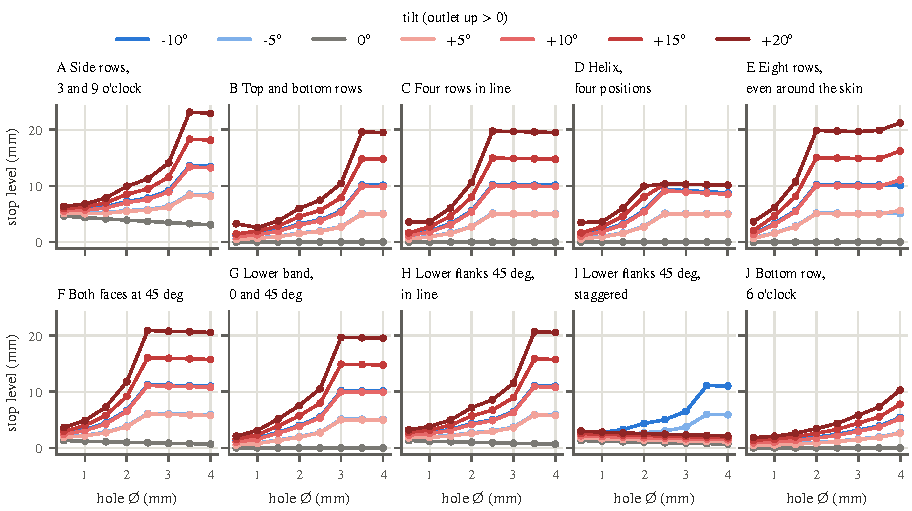
\includegraphics[width=\linewidth]{fig09_hstop_vs_d_area.pdf}
\caption{Stop level against hole diameter, fixed-area family (about 28\,mm$^2$). Larger holes mean fewer stations; above about 2.5\,mm the holes no longer reach the ends of the drain.}
\label{fig:harea}
\end{figure}

\begin{figure}[!htbp]
\centering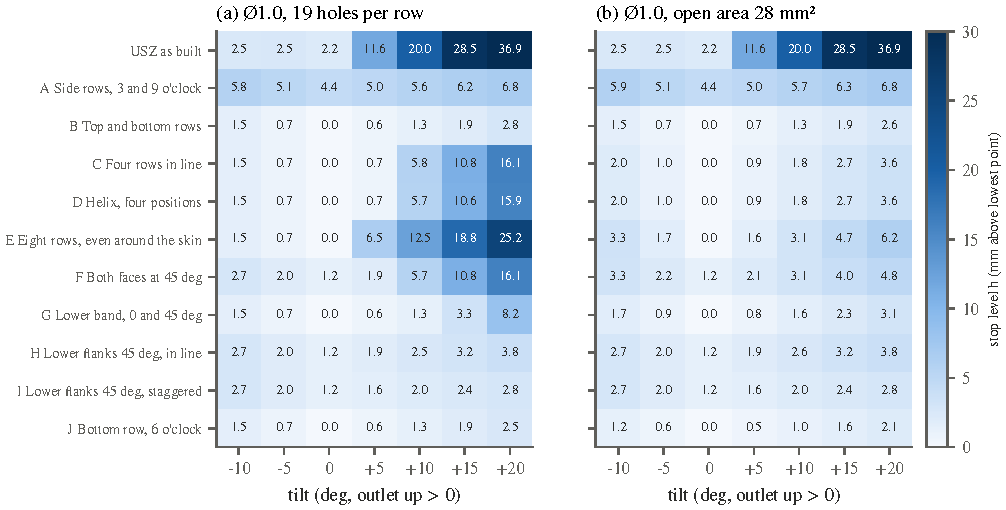
\includegraphics[width=\linewidth]{fig10_heatmap_tilt.pdf}
\caption{Stop level (mm) for every layout with \O1.0\,mm holes and tilts from $-10^\circ$ to $+20^\circ$. (a) 19 holes per row. (b) Open area of about 28\,mm$^2$.}
\label{fig:heat}
\end{figure}

\begin{table}[!htbp]
\centering\footnotesize
\caption{Stop level $h_s$ (mm) of all layouts with \O1.0\,mm holes at about 28\,mm$^2$ open area (USZ as built), from the network simulation. $Q_0$ is the flow with the pool 3\,mm above the drain.}\label{tab:layouts}
\setlength{\tabcolsep}{4pt}
\begin{tabular}{@{}l r r rrrrrrr@{}}
\toprule
 & & & \multicolumn{7}{c}{stop level $h_s$ (mm) at tilt $\alpha$} \\
\cmidrule(l){4-10}
layout & $A$ (mm$^2$) & $Q_0$ (mL/min) & $-10^\circ$ & $-5^\circ$ & $0^\circ$ & $+5^\circ$ & $+10^\circ$ & $+15^\circ$ & $+20^\circ$ \\
\midrule
USZ as built (318 $\times$ \O1.0) & 468 & 965 & 2.5 & 2.5 & 2.2 & 11.6 & 20.0 & 28.5 & 36.9 \\
A\ \ Side rows, 3 and 9 o'clock & 28 & 755 & 5.9 & 5.1 & 4.4 & 5.0 & 5.7 & 6.3 & 6.8 \\
B\ \ Top and bottom rows & 28 & 755 & 1.5 & 0.7 & 0.0 & 0.7 & 1.3 & 1.9 & 2.6 \\
C\ \ Four rows in line & 28 & 755 & 2.0 & 1.0 & 0.0 & 0.9 & 1.8 & 2.7 & 3.6 \\
D\ \ Helix, four positions & 28 & 755 & 2.0 & 1.0 & 0.0 & 0.9 & 1.8 & 2.7 & 3.6 \\
E\ \ Eight rows, even around the skin & 25 & 721 & 3.3 & 1.7 & 0.0 & 1.6 & 3.1 & 4.7 & 6.2 \\
F\ \ Both faces at 45$^\circ$ & 28 & 755 & 3.3 & 2.2 & 1.2 & 2.1 & 3.1 & 4.0 & 4.8 \\
G\ \ Lower band, 0 and 45$^\circ$ & 28 & 755 & 1.7 & 0.9 & 0.0 & 0.8 & 1.6 & 2.3 & 3.1 \\
H\ \ Lower flanks 45$^\circ$, in line & 28 & 755 & 2.7 & 2.0 & 1.2 & 1.9 & 2.6 & 3.2 & 3.8 \\
I\ \ Lower flanks 45$^\circ$, staggered & 28 & 755 & 2.7 & 2.0 & 1.2 & 1.6 & 2.0 & 2.4 & 2.8 \\
J\ \ Bottom row, 6 o'clock & 28 & 755 & 1.2 & 0.6 & 0.0 & 0.5 & 1.0 & 1.6 & 2.1 \\
\midrule
\textbf{Recommended}, $\pm30^\circ$ staggered & 28 & 755 & 2.0 & 1.3 & 0.5 & 0.9 & 1.4 & 1.8 & 2.1 \\
\bottomrule
\end{tabular}

\end{table}

\subsection{Optimising the layout}\label{sec:opt}
Two staggered rows were then mapped over hole size (0.5 to 4\,mm) and number of holes (Fig.~\ref{fig:opt}). Flow when submerged rises with open area and reaches 80\,\% of $Q_{max}$ at about $2A_p$ (Fig.~\ref{fig:opt}a, Fig.~\ref{fig:design}b). The worst stop level over $-10^\circ$ to $+15^\circ$ has a broad minimum between about 15 and 40\,mm$^2$ (Fig.~\ref{fig:opt}b):
\begin{itemize}
\item With less area there are too few holes to reach the ends.
\item With more area, $\Lw$ exceeds $\Lambda^*$ (Eq.~\eqref{eq:lstar}), and the lift fails at outlet-up tilts.
\end{itemize}
The rows should sit as low as practical (Fig.~\ref{fig:opt}c): every $15^\circ$ lower takes 0.5 to 1\,mm off the residual level. However, rows below about $\pm20^\circ$ press against a floor or against tissue (when lying on a hard floor, the holes at $\pm15^\circ$ lose 70\,\% of their flow). We therefore chose $\pm30^\circ$, roughly 5 and 7 o'clock. At a fixed area of 28\,mm$^2$ (Table~\ref{tab:sizes}), holes of 1.0 to 1.5\,mm give the best balance:
\begin{itemize}
\item 0.5\,mm holes lose flow to viscosity and clog easily.
\item 2 to 4\,mm holes come in too few stations and leave the outlet end uncovered when it is lowest.
\end{itemize}

\begin{figure}[!htbp]
\centering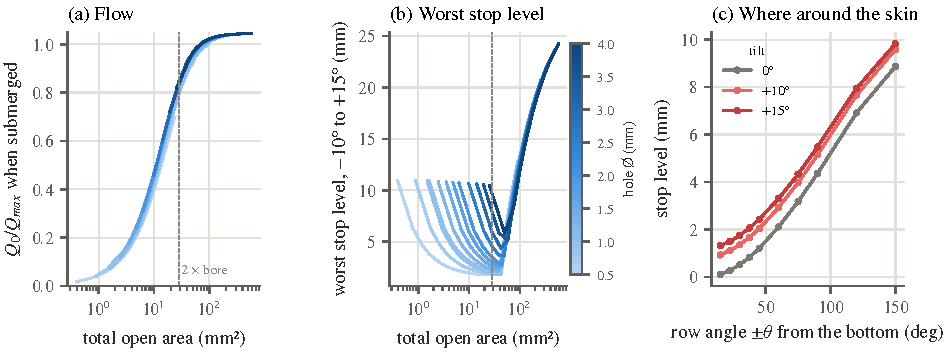
\includegraphics[width=\linewidth]{fig12_optimize.pdf}
\caption{Optimisation of two staggered rows at $\pm30^\circ$. Each line is one hole size, with the number of holes varied along it. (a) Flow when submerged as a fraction of the bore limit. (b) Worst stop level over $-10^\circ$ to $+15^\circ$ (closed form). The ring marks the recommended design, and the dashed line is twice the bore area. (c) Effect of the row angle $\pm\theta$ (\O1.0\,mm, 28 holes).}
\label{fig:opt}
\end{figure}

\begin{figure}[!htbp]
\centering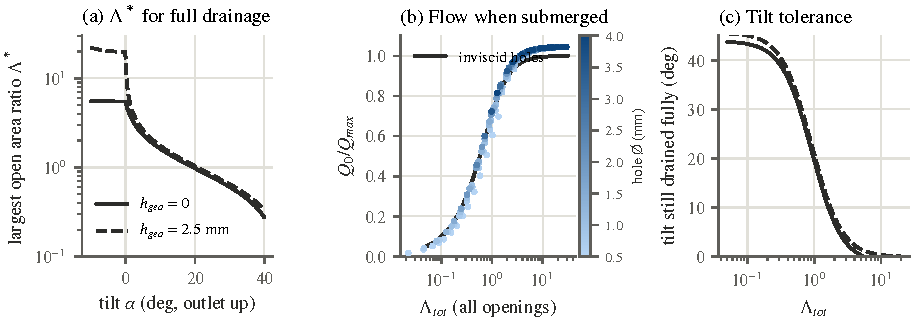
\includegraphics[width=\linewidth]{fig06_design_chart.pdf}
\caption{Closed-form design charts. (a) Largest exposed-area ratio that still drains to the lowest hole, Eq.~\eqref{eq:lstar}. (b) Flow when submerged against total area ratio (line: inviscid holes in series with the bore; dots: network results, coloured by hole size). (c) Largest outlet-up tilt that still drains fully, if all holes are exposed at the end.}
\label{fig:design}
\end{figure}

\begin{table}[!htbp]
\centering\small
\caption{Recommended layout (two staggered rows at $\pm30^\circ$) at about 28\,mm$^2$ for each hole size: stop level $h_s$ (mm).}\label{tab:sizes}
\begin{tabular}{@{}r r r r rrrrrrr@{}}
\toprule
\O\ (mm) & holes & $A$ (mm$^2$) & $Q_0$ (mL/min) & $-10^\circ$ & $-5^\circ$ & $0^\circ$ & $+5^\circ$ & $+10^\circ$ & $+15^\circ$ & $+20^\circ$ \\
\midrule
{0.5} & 144 & 28 & 699 & 1.7 & 1.2 & 0.6 & 1.0 & 1.4 & 1.9 & 2.3 \\
\textbf{1} & 36 & 28 & 755 & 2.0 & 1.3 & 0.5 & 0.9 & 1.4 & 1.8 & 2.1 \\
{1.5} & 16 & 28 & 773 & 2.6 & 1.6 & 0.5 & 0.9 & 1.3 & 1.7 & 2.0 \\
{2} & 8 & 25 & 747 & 3.7 & 2.1 & 0.4 & 0.8 & 1.2 & 1.6 & 1.9 \\
{2.5} & 6 & 29 & 794 & 4.4 & 2.4 & 0.3 & 0.8 & 1.2 & 1.5 & 1.8 \\
{3} & 4 & 28 & 786 & 5.9 & 3.2 & 0.3 & 0.7 & 1.1 & 1.4 & 1.7 \\
{3.5} & 2 & 19 & 670 & 10.6 & 5.5 & 0.3 & 0.7 & 1.0 & 1.4 & 1.6 \\
{4} & 2 & 25 & 756 & 10.5 & 5.4 & 0.2 & 0.6 & 1.0 & 1.3 & 1.5 \\
\bottomrule
\end{tabular}

\end{table}

\subsection{How far can the drain be tilted?}
Figure~\ref{fig:tilt} extends the tilt to $40^\circ$. With the outlet down, all layouts stop within about 3\,mm of the bottom (side rows excepted). With the outlet up, the recommended design drains to its lowest hole edge up to $\alpha=\numrecTiltLimit^\circ$. Beyond that, $\zl$ grows faster than the vacuum can lift, and the stop level rises by about 1\,mm per degree. The as-built USZ field fails from the first degree of outlet-up tilt.

\begin{figure}[!htbp]
\centering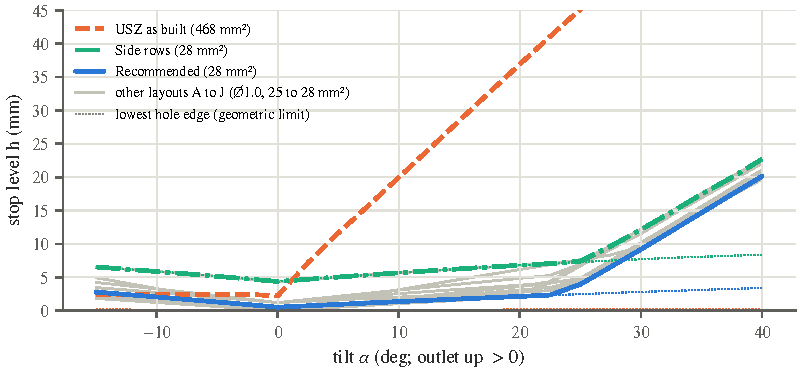
\includegraphics[width=\linewidth]{fig16_tiltlimit.pdf}
\caption{Stop level against tilt from $-15^\circ$ to $+40^\circ$. Dotted lines mark the lowest hole edge, i.e. the best any layout can do.}
\label{fig:tilt}
\end{figure}

\subsection{When the source has limited capacity}
The results so far assume a regulator that holds $-7$\,mmHg whatever the air flow. Once the recommended drain is fully exposed it draws about \numairLo{} to \numairHi\,L/min of air, and the USZ field about 28\,L/min. For the recommended layout, the smallest source capacity that still drains to the lowest hole is \numcapFive, \numcapTen, \numcapFifteen{} and \numcapTwenty\,L/min at $+5^\circ$, $+10^\circ$, $+15^\circ$ and $+20^\circ$. This is the free-air flow a wall regulator must pass while holding $-7$\,mmHg. If the source moves less than that, its vacuum collapses while holes are exposed, and with the outlet up the drain stops early (Fig.~\ref{fig:pump}, Table~\ref{tab:pump}). Equation~\eqref{eq:cap-area} gives a conservative estimate of the allowed open area. A 10\,L/min source allows about 16 to 19\,mm$^2$, and a 5\,L/min source about 9\,mm$^2$. A layout fitted to the source capacity drains to the bottom again; when lying flat ($\zl=2.7$\,mm) the source capacity makes no difference.

\begin{figure}[!htbp]
\centering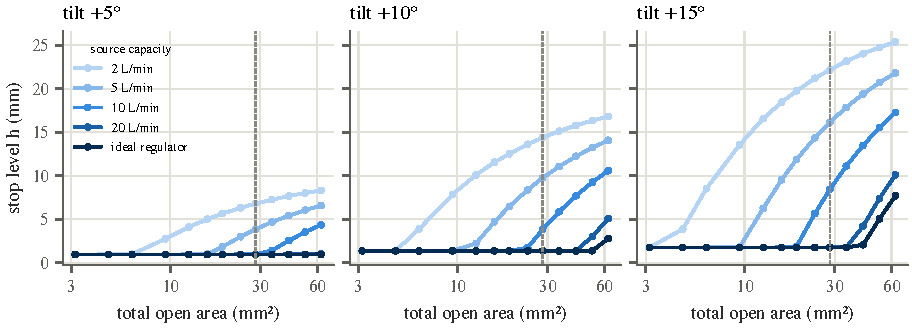
\includegraphics[width=\linewidth]{fig17_pump.pdf}
\caption{Stop level against total open area (recommended layout, \O1.0\,mm) for sources of limited flow capacity. The dashed line is twice the bore area.}
\label{fig:pump}
\end{figure}

\begin{table}[!htbp]
\centering\small
\caption{Largest total open area (recommended layout, \O1.0\,mm) that still drains to the lowest hole, against source capacity: network simulation and the conservative estimate of Eq.~\eqref{eq:cap-area}.}\label{tab:pump}
\begin{tabular}{@{}l r r r r@{}}
\toprule
source capacity & \multicolumn{2}{c}{largest open area that still drains fully (mm$^2$)} & \multicolumn{2}{c}{Eq.~\eqref{eq:cap-area} (mm$^2$)} \\
\cmidrule(lr){2-3}\cmidrule(l){4-5}
 & $\alpha=+10^\circ$ & $\alpha=+15^\circ$ & $+10^\circ$ & $+15^\circ$ \\
\midrule
2 L/min & 5 & 3 & 3 & 2 \\
5 L/min & 9 & 9 & 7 & 6 \\
10 L/min & 19 & 16 & 14 & 11 \\
20 L/min & 42 & 35 & 27 & 23 \\
ideal regulator & 52 & 35 & -- & -- \\
\bottomrule
\end{tabular}

\end{table}

\subsection{Sensitivity and robustness}
Table~\ref{tab:sens} and Fig.~\ref{fig:sens} vary one assumption at a time:
\begin{itemize}
\item \textbf{Liquid and suction level.} Viscosity (water to 80\,\% glycerol), suction ($-5$ to $-10$\,mmHg) and the discharge coefficients change the flow rates but hardly the stop levels, because the stop is set by gas flow and hydrostatics.
\item \textbf{Capillary holding.} It does not change the recommended design, which already drains fully, but it would help the as-built USZ field a lot (20 down to 3.6\,mm at $10^\circ$ with perfect wetting), because many small wetted holes can hold back air once the vacuum has dropped. The tube material and surface state matter here.
\item \textbf{Drawdown.} Surface drawdown above active holes adds about half a hole diameter to every stop level.
\item \textbf{Lying on a floor.} This blocks the bottom row of layout C, which then stops at mid-height (layout J would be blocked entirely). The recommended rows at $\pm30^\circ$ are not affected.
\end{itemize}
In a Monte Carlo study ($\numnMC$ random combinations of tilt from $-10^\circ$ to $+15^\circ$, suction, liquid, discharge coefficients, contact angle and drawdown; Fig.~\ref{fig:mc}), the recommended design had a median stop level of \nummcRecMed\,mm and a 95th percentile of \nummcRecPnf\,mm. For the as-built USZ field these were \nummcUszMed\,mm and \nummcUszPnf\,mm.

\begin{figure}[!htbp]
\centering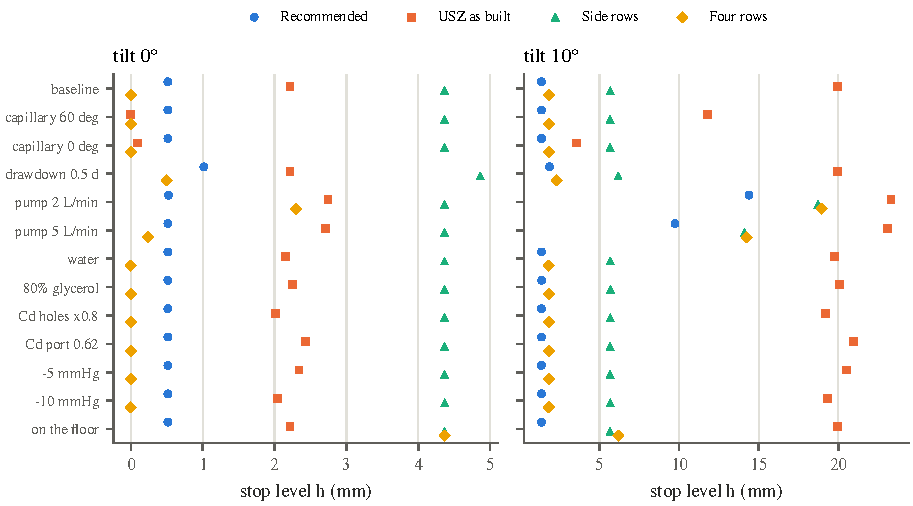
\includegraphics[width=\linewidth]{fig14_sensitivity.pdf}
\caption{One-at-a-time sensitivity of the stop level, flat (left) and outlet $10^\circ$ up (right).}
\label{fig:sens}
\end{figure}

\begin{table}[!htbp]
\centering\footnotesize
\caption{Sensitivity: stop level $h_s$ (mm) at $0^\circ$ and $+10^\circ$.}\label{tab:sens}
\setlength{\tabcolsep}{4pt}
\begin{tabular}{@{}l r r r r r r r r @{}}
\toprule
case & \multicolumn{2}{c}{Recommended} & \multicolumn{2}{c}{USZ as built} & \multicolumn{2}{c}{Side rows} & \multicolumn{2}{c}{Four rows} \\
\cmidrule(lr){2-3}\cmidrule(lr){4-5}\cmidrule(lr){6-7}\cmidrule(lr){8-9}
 & $0^\circ$ & $+10^\circ$ & $0^\circ$ & $+10^\circ$ & $0^\circ$ & $+10^\circ$ & $0^\circ$ & $+10^\circ$ \\
\midrule
baseline & 0.5 & 1.4 & 2.2 & 20.0 & 4.4 & 5.7 & 0.0 & 1.8 \\
capillary 60 deg & 0.5 & 1.4 & 0.0 & 11.8 & 4.4 & 5.7 & 0.0 & 1.8 \\
capillary 0 deg & 0.5 & 1.4 & 0.1 & 3.6 & 4.4 & 5.7 & 0.0 & 1.8 \\
drawdown 0.5 d & 1.0 & 1.9 & 2.2 & 20.0 & 4.9 & 6.2 & 0.5 & 2.3 \\
pump 2 L/min & 0.5 & 14.4 & 2.7 & 23.3 & 4.4 & 18.7 & 2.3 & 18.9 \\
pump 5 L/min & 0.5 & 9.7 & 2.7 & 23.1 & 4.4 & 14.1 & 0.2 & 14.2 \\
water & 0.5 & 1.4 & 2.2 & 19.7 & 4.4 & 5.7 & 0.0 & 1.8 \\
80\% glycerol & 0.5 & 1.4 & 2.2 & 20.1 & 4.4 & 5.7 & 0.0 & 1.8 \\
Cd holes x0.8 & 0.5 & 1.4 & 2.0 & 19.2 & 4.4 & 5.7 & 0.0 & 1.8 \\
Cd port 0.62 & 0.5 & 1.4 & 2.4 & 20.9 & 4.4 & 5.7 & 0.0 & 1.8 \\
-5 mmHg & 0.5 & 1.4 & 2.3 & 20.5 & 4.4 & 5.7 & 0.0 & 1.8 \\
-10 mmHg & 0.5 & 1.4 & 2.0 & 19.3 & 4.4 & 5.7 & 0.0 & 1.8 \\
on the floor & 0.5 & 1.4 & 2.2 & 19.9 & 4.4 & 5.7 & 4.4 & 6.2 \\
\bottomrule
\end{tabular}

\end{table}

\begin{figure}[!htbp]
\centering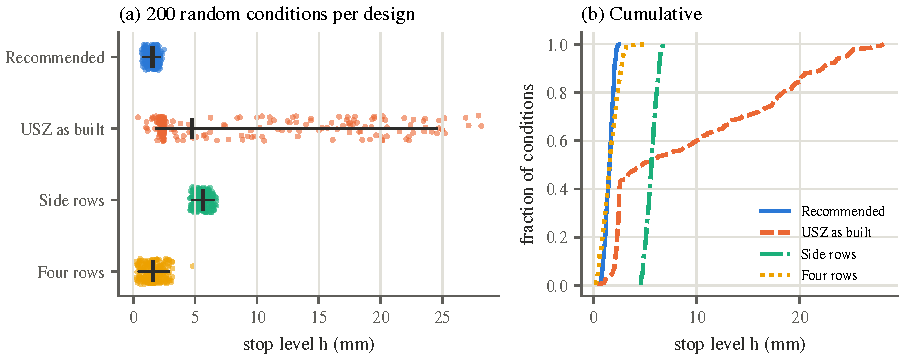
\includegraphics[width=\linewidth]{fig15_montecarlo.pdf}
\caption{Monte Carlo study: stop level under $\numnMC$ random operating conditions per design. (a) Each dot is one condition; the bars show the median and the 5th to 95th percentiles. (b) Cumulative distributions.}
\label{fig:mc}
\end{figure}


\FloatBarrier
% =============================================================================
\section{Recommended design}\label{sec:design}
\begin{table}[H]
\centering\small
\caption{Recommended hole layout for the USZ body at $-7$\,mmHg.}\label{tab:rec}
\begin{tabular}{@{}l p{0.62\linewidth}@{}}
\toprule
rows & two rows at $\theta=\pm30^\circ$ from the bottom line (about 5 and 7 o'clock when lying flat); none on the upper half \\
alignment & staggered by half a pitch \\
holes & \O1.0\,mm (1.0 to 1.5\,mm is equally good), 18 per row, pitch 6.0\,mm \\
span & $x=5$ to $113$\,mm, reaching as close to both ends as the part allows \\
open area & \numrecArea\,mm$^2$ $\approx2\times$ bore area ($\Lambda_{tot}=\numrecLam$) \\
suction source & wall regulator holding $-7$\,mmHg while passing \numcapTwenty\,L/min of air (\numcapTen\,L/min up to $10^\circ$ tilt); with a 5 to 10\,L/min source, reduce to 12 to 24 holes (Table~\ref{tab:pump}) \\
expected stop level & \numrecHmin\,mm (flat) to \numrecHmax\,mm ($20^\circ$), i.e. the lowest hole edge; full drainage up to $\numrecTiltLimit^\circ$ \\
flow when submerged & \numrecQ\,mL/min (\numrecQfrac\,\% of the bore limit) \\
\bottomrule
\end{tabular}
\end{table}

\noindent The design rules, in order of importance:
\begin{enumerate}
\item Keep the total open area near 1 to 2 times the bore area. More area adds almost no flow, because the bore already limits it, but it destroys the vacuum once holes are exposed.
\item Put the holes on the lower half of the skin, but not on the contact line.
\item Spread them uniformly along the whole length, using small holes so that there are enough stations to reach both ends, and stagger the rows.
\item Match the open area to the flow capacity of the suction source.
\end{enumerate}
A flat drain may come to rest upside down. Mirroring the rows onto the top face would double the exposed area and cost tilt tolerance, so marking the orientation is the better fix.

\paragraph{Suggested bench test.} In the glycerol--water tank:
\begin{itemize}
\item tilt the drain to $0^\circ$, $5^\circ$, $10^\circ$ and $15^\circ$ with the outlet up, and record the residual level;
\item measure the vacuum in the outlet tube close to the drain, to confirm that the wall regulator really holds $-7$\,mmHg while the drain sucks air (about \numairHi\,L/min);
\item compare the as-built USZ part with a part drilled to Table~\ref{tab:rec}.
\end{itemize}
The model predicts that at $10^\circ$ the as-built part leaves about 20\,mm and the recommended part about 1.4\,mm.

% =============================================================================
\section{Three-dimensional CFD check}\label{sec:cfd}
The network model represents each opening and the bore by flow laws, and the inside of the drain by one gas pressure and one flat liquid level. A three-dimensional two-phase simulation drops these simplifications. It resolves the jets through the openings, the shape of the liquid inside the drain, the air stream into the bore and the actual pressure field. One case was run for each layout (Table~\ref{tab:cfd}). The set-up, all pictures and animations, and the logged data are in \texttt{vof/kratos/}.

\paragraph{Solver and geometry.} The solver is the two-fluid Navier--Stokes solver of Kratos Multiphysics~10.3. The flow is laminar, both phases are incompressible, and a level set tracks the liquid--air interface. Surface tension is not modelled, which matches the model's base case (contact angle $90^\circ$). The fluid properties are those of Section~\ref{sec:geometry}.

The geometry is built with gmsh/OpenCASCADE from the model's geometry: every opening drilled through the 0.6\,mm wall along the skin normal, the \O4.24\,mm bore in the end face, and a 16.8\,mm outlet tube. The drain sits in a trough 5.5\,mm wider than it on each side, with a floor 2.5\,mm below the drain and parallel to it (Fig.~\ref{fig:cfd-domain}). The mesh is built in the drain frame, and the $10^\circ$ tilt enters only through gravity. The boundary conditions are:
\begin{itemize}
\item \textbf{Outlet:} the pressure at the tube end is held at $-933$\,Pa, an ideal wall regulator.
\item \textbf{Top of the trough:} open to the atmosphere (0\,Pa), so air can flow in and out.
\item \textbf{All walls:} no-slip.
\end{itemize}

\paragraph{Mesh and time step.} The tetrahedral mesh has these cell sizes (as-built field in brackets):
\begin{itemize}
\item 0.25\,mm (0.35\,mm) at the opening rims and the bore;
\item 0.5\,mm (0.6\,mm) on the skin;
\item 0.8\,mm inside the drain;
\item 1.6\,mm in the pool and the air.
\end{itemize}
This gives 139\,k nodes and 645\,k cells for the recommended layout, and 203\,k nodes and 827\,k cells for the as-built field.

The time step is fixed at 50\,\textmu s (implicit BDF2). Kratos's default acceleration limit of $5\,g$ is switched off: the air jets through the openings accelerate at about $10^5$\,m/s$^2$, and the limit stops them. On a 12-core laptop one step takes 25--60\,s.

\paragraph{Fixed-level snapshots.} A full drainage takes seconds of flow time, which would need weeks on this machine, so each run is a snapshot at one pool level $h$:
\begin{itemize}
\item \textbf{Start:} the pool starts at $h$. The drain interior starts filled to the inner level $\zeta(h)$ that the model predicts, with air above it.
\item \textbf{Logged every step:} the liquid and air flow at the outlet, and the pressure at eight probes along the top of the interior and in the bore.
\item \textbf{Saved every 5\,ms:} the full fields.
\item \textbf{Flow through each opening:} sampled on a disc across the middle of its bore.
\end{itemize}

\begin{table}[H]
\centering\small
\caption{The two CFD cases at $\alpha=10^\circ$. CFD values are averaged over the flow-time window shown; the model's prediction is at the same pool level. The pressure is taken at the top of the drain interior, in its last 30\,mm before the end face.}\label{tab:cfd}
\begin{tabular}{@{}l r r r r r r@{}}
\toprule
 & pool & stop level & window & liquid out & air out & interior pressure \\
 & (mm) & (mm) & (ms) & (mL/min) & (L/min) & (Pa) \\
\midrule
recommended layout, CFD & 8 & -- & 40--50 & 674 & 0.05 & $-60$ to $-90$ (in liquid) \\
\quad model & 8 & 1.4 & -- & 203 & 14.7 & $-427$ \\[1mm]
USZ as built, CFD & 21 & -- & 4--15 & 58 & 16.5 & $-5$ to $-85$ (in air) \\
\quad model & 21 & 20.0 & -- & 148 & 23.3 & $-37.5$ \\
\bottomrule
\end{tabular}
\end{table}

\begin{figure}[!htbp]
\centering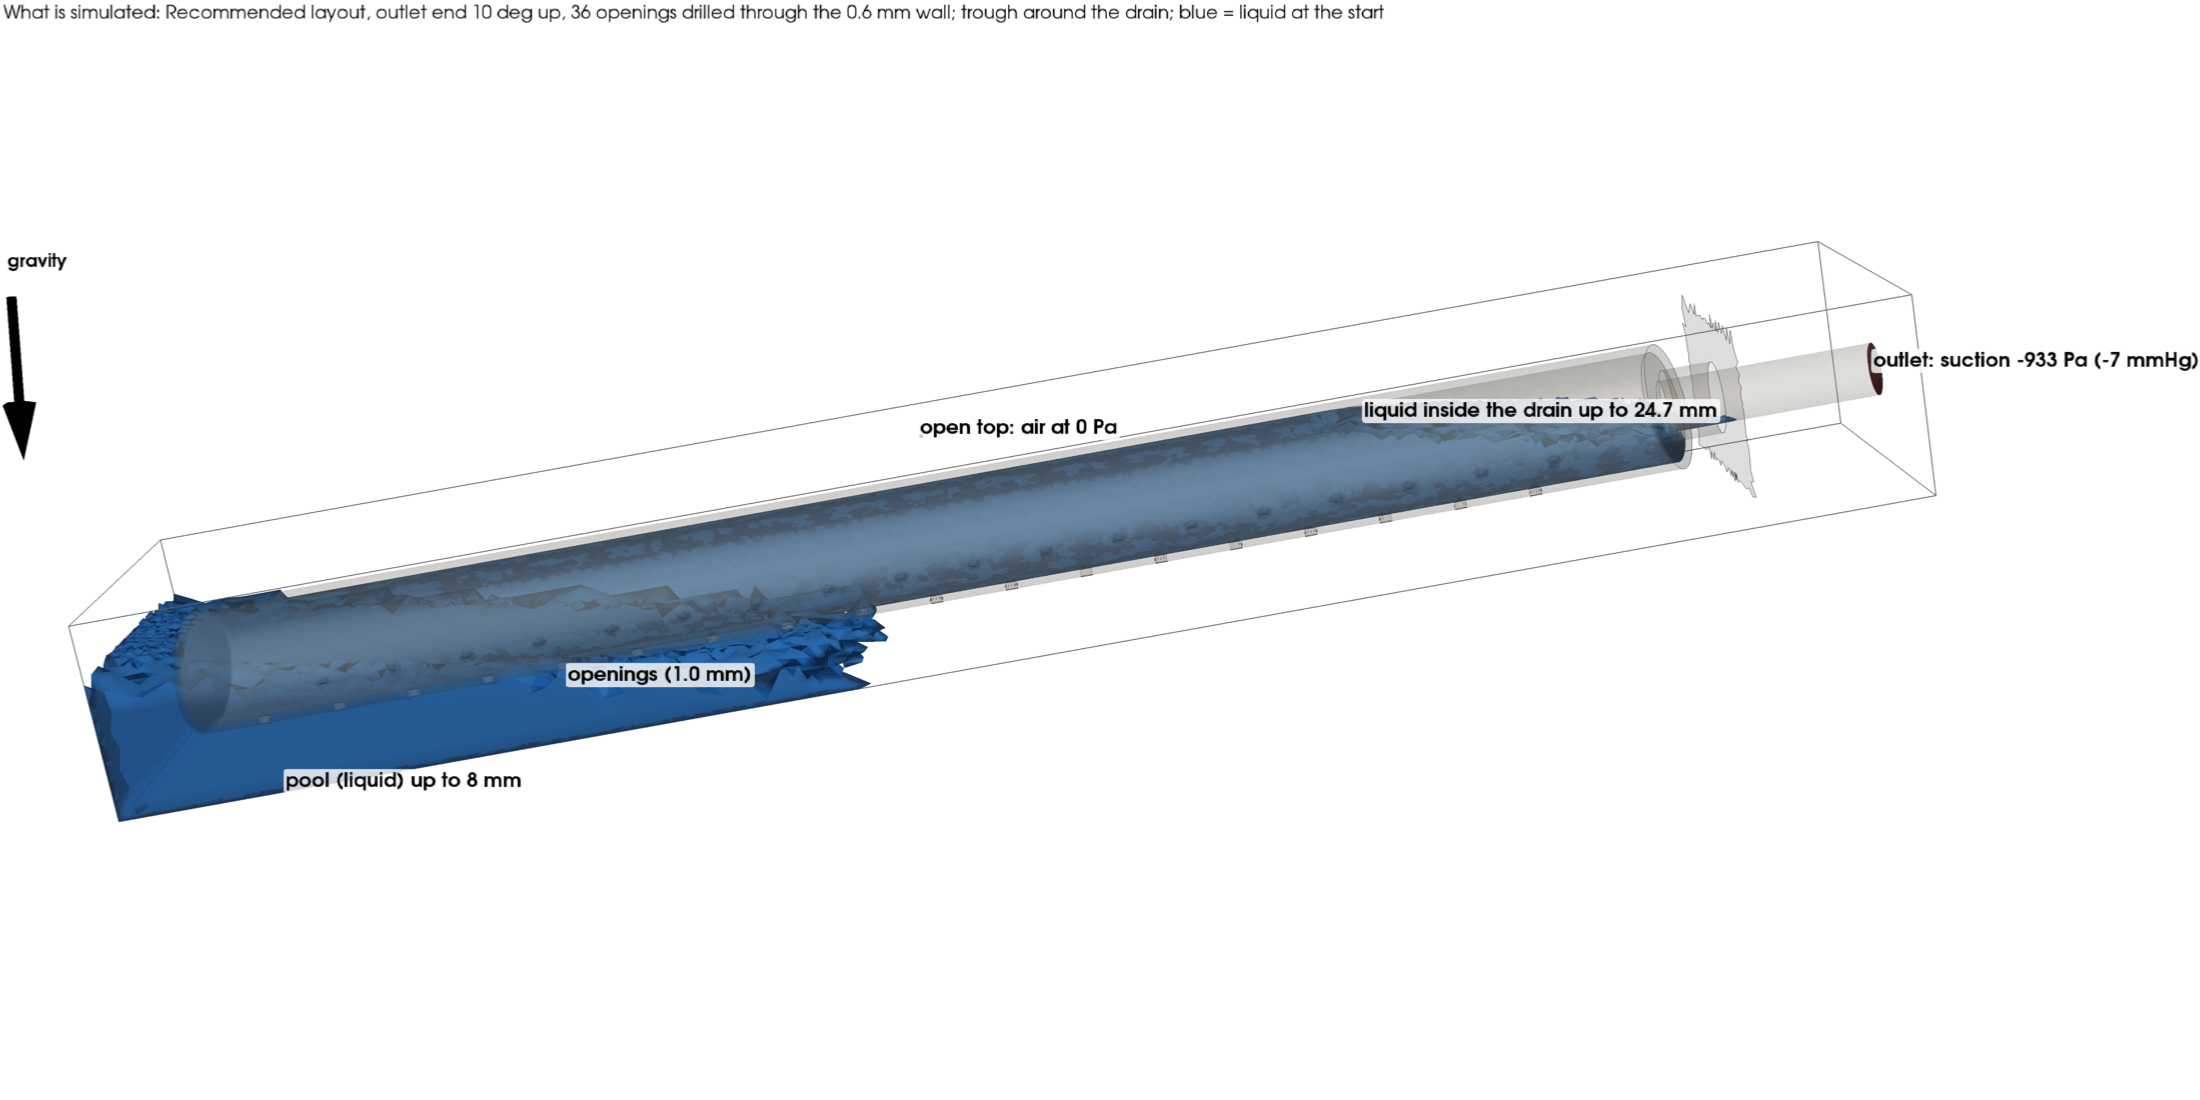
\includegraphics[width=0.85\linewidth]{cfd_rec_setup.png}
\caption{CFD set-up of the recommended-layout case: the drain in its trough with the outlet end $10^\circ$ up, the pool at 8\,mm, and the liquid inside the drain at the model's inner level.}
\label{fig:cfd-domain}
\end{figure}

\paragraph{As-built field, pool at 21\,mm.} This level is 1\,mm above the model's stop level.
\begin{itemize}
\item \textbf{Air:} within 2\,ms the air flow through the exposed openings rises to 16--17\,L/min and stays there (Fig.~\ref{fig:cfd-usz}). The flows sampled in the 609 openings add up to 16.5\,L/min of air, the same as at the outlet.
\item \textbf{Liquid:} it leaves only as a thin film and in short slugs, 58\,mL/min on average. The openings take in 45\,mL/min.
\item \textbf{Inside the drain:} the liquid stays near the model's inner level ($\zeta=24.3$\,mm), about 3\,mm above the pool, held up by the vacuum. The air flows along the top of the interior into the bore at several metres per second.
\item \textbf{Air pressure:} along the top of the interior it falls from about $-5$\,Pa, 30\,mm before the end face, to $-85$\,Pa just before the bore. The model's single gas pressure, $-37.5$\,Pa, lies in between.
\end{itemize}
The CFD therefore shows the state the model predicts near the stop: the outlet carries mainly air and little liquid. The air flow is 29\,\% below the model's value.

At 16.4\,ms a liquid slug reached the end of the outlet tube, where the pressure is prescribed, and the solution diverged numerically. The fields up to 15\,ms come before this and are used here.

\begin{figure}[!htbp]
\centering
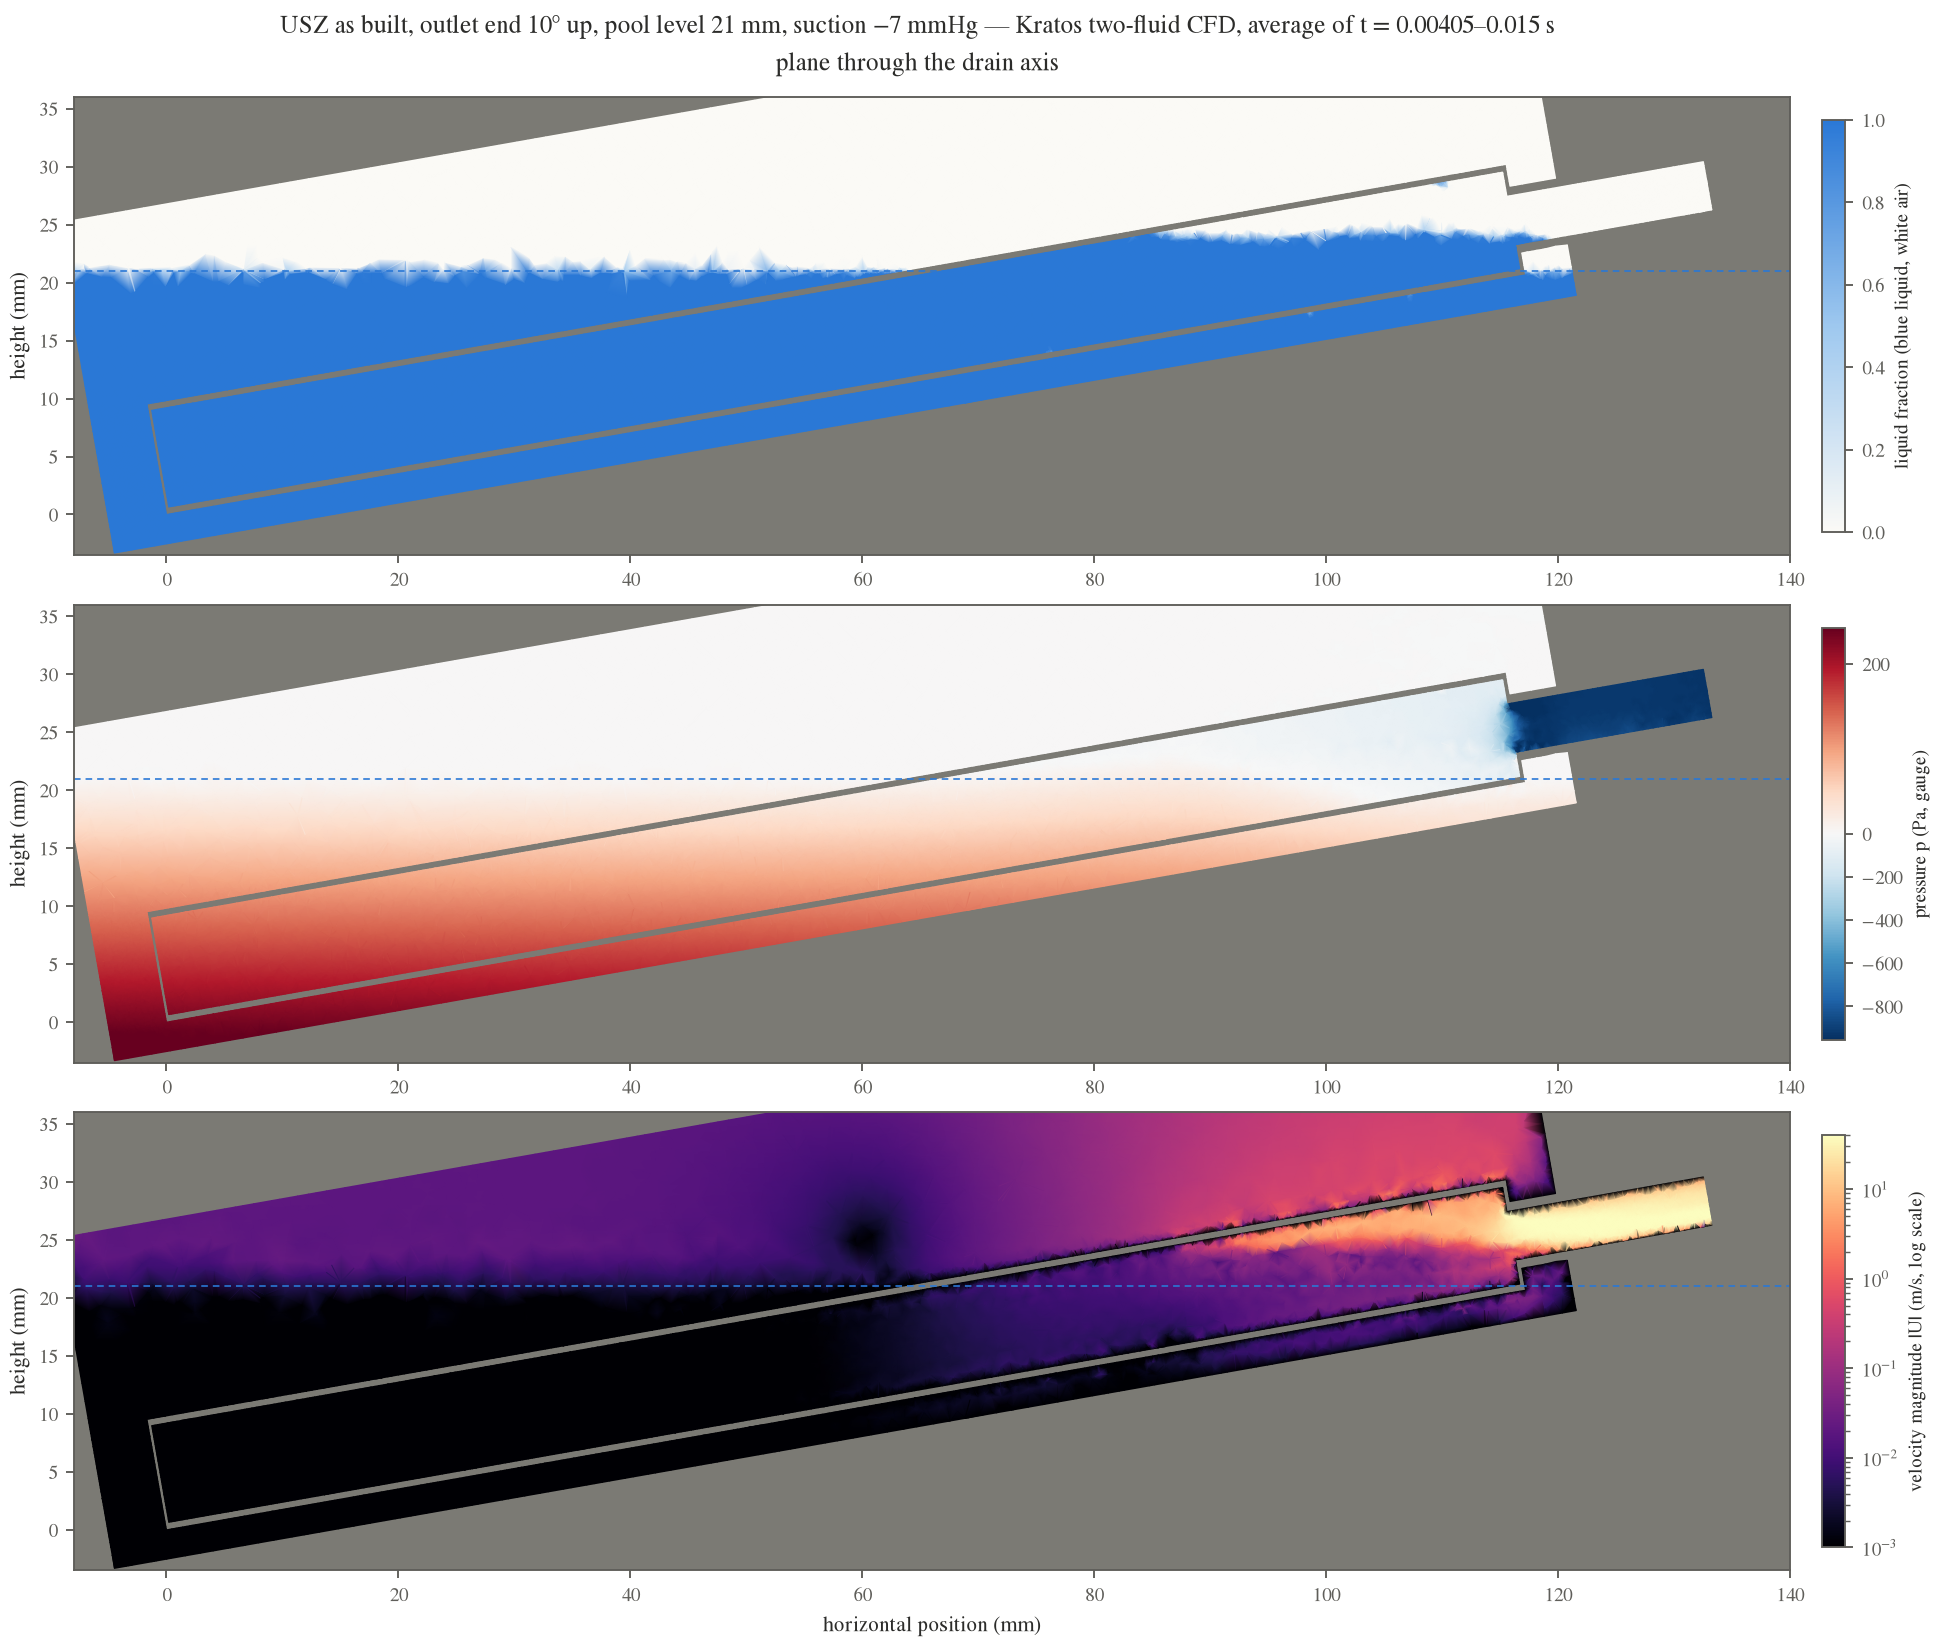
\includegraphics[width=\linewidth]{cfd_usz_midplane.png}\\[2mm]
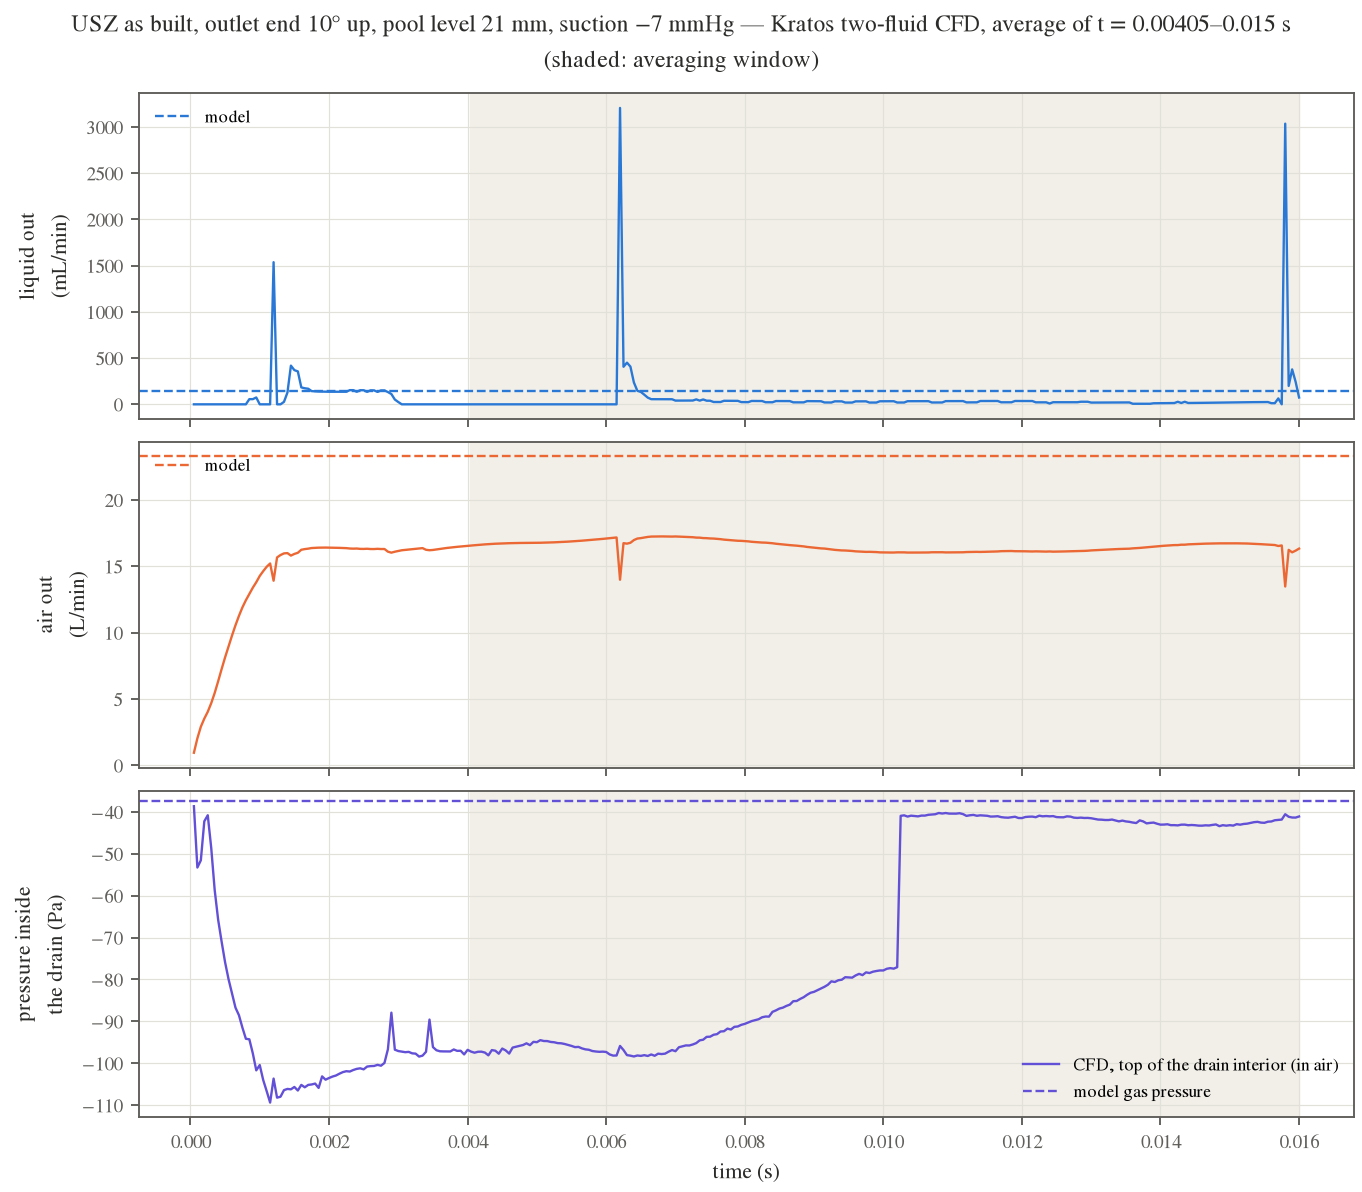
\includegraphics[width=0.8\linewidth]{cfd_usz_history.png}
\caption{As-built field, pool at 21\,mm. Top: the plane through the drain axis, averaged over 4--15\,ms; it shows the liquid (blue), the pressure, and the speed on a log scale. Bottom: the liquid and air flow at the outlet and the air pressure at the top of the interior against time, with the model's values dashed. The step in the pressure at 10.2\,ms is where a second probe comes out of the liquid into the air.}
\label{fig:cfd-usz}
\end{figure}

\paragraph{Recommended layout, pool at 8\,mm.} This run did not reach a steady state in the 50\,ms computed. It went through three stages:
\begin{enumerate}
\item \textbf{Start (0--12\,ms).} With $\zeta=24.7$\,mm, the drain starts 94\,\% full of liquid. The air pocket left at the top of the outlet end is held at $-650$ to $-900$\,Pa (model: $-427$\,Pa), and air leaves at 4--6\,L/min (model: 14.7\,L/min).
\item \textbf{Priming (12--37\,ms).} The pocket is drawn off and the bore fills with liquid. Air then enters only as bubbles through the exposed openings (Fig.~\ref{fig:cfd-rec}).
\item \textbf{Siphon (37--50\,ms).} The outlet carries 674\,mL/min of liquid and almost no air, and the pressure at the top of the interior, now in liquid, is only $-60$ to $-90$\,Pa.
\end{enumerate}
That vacuum can't hold the liquid column 16.7\,mm above the pool, which needs at least $-184$\,Pa. So the drain is emptying the liquid it started with, not drawing it from the pool:
\begin{itemize}
\item at 50\,ms its lowest openings carry liquid outward into the pool, at 0.4--0.5\,m/s (about 10\,mL/min each);
\item the liquid inside the drain fell from 12.35 to 12.11\,mL between 5 and 50\,ms;
\item only 0.21\,mL left through the outlet in the whole run.
\end{itemize}
The outlet flow at 50\,ms is therefore part of the start-up, and it can't be compared with the model's steady 203\,mL/min. Reaching the steady state would take a few tenths of a second of flow, that is two to three days on this laptop.

\begin{figure}[!htbp]
\centering
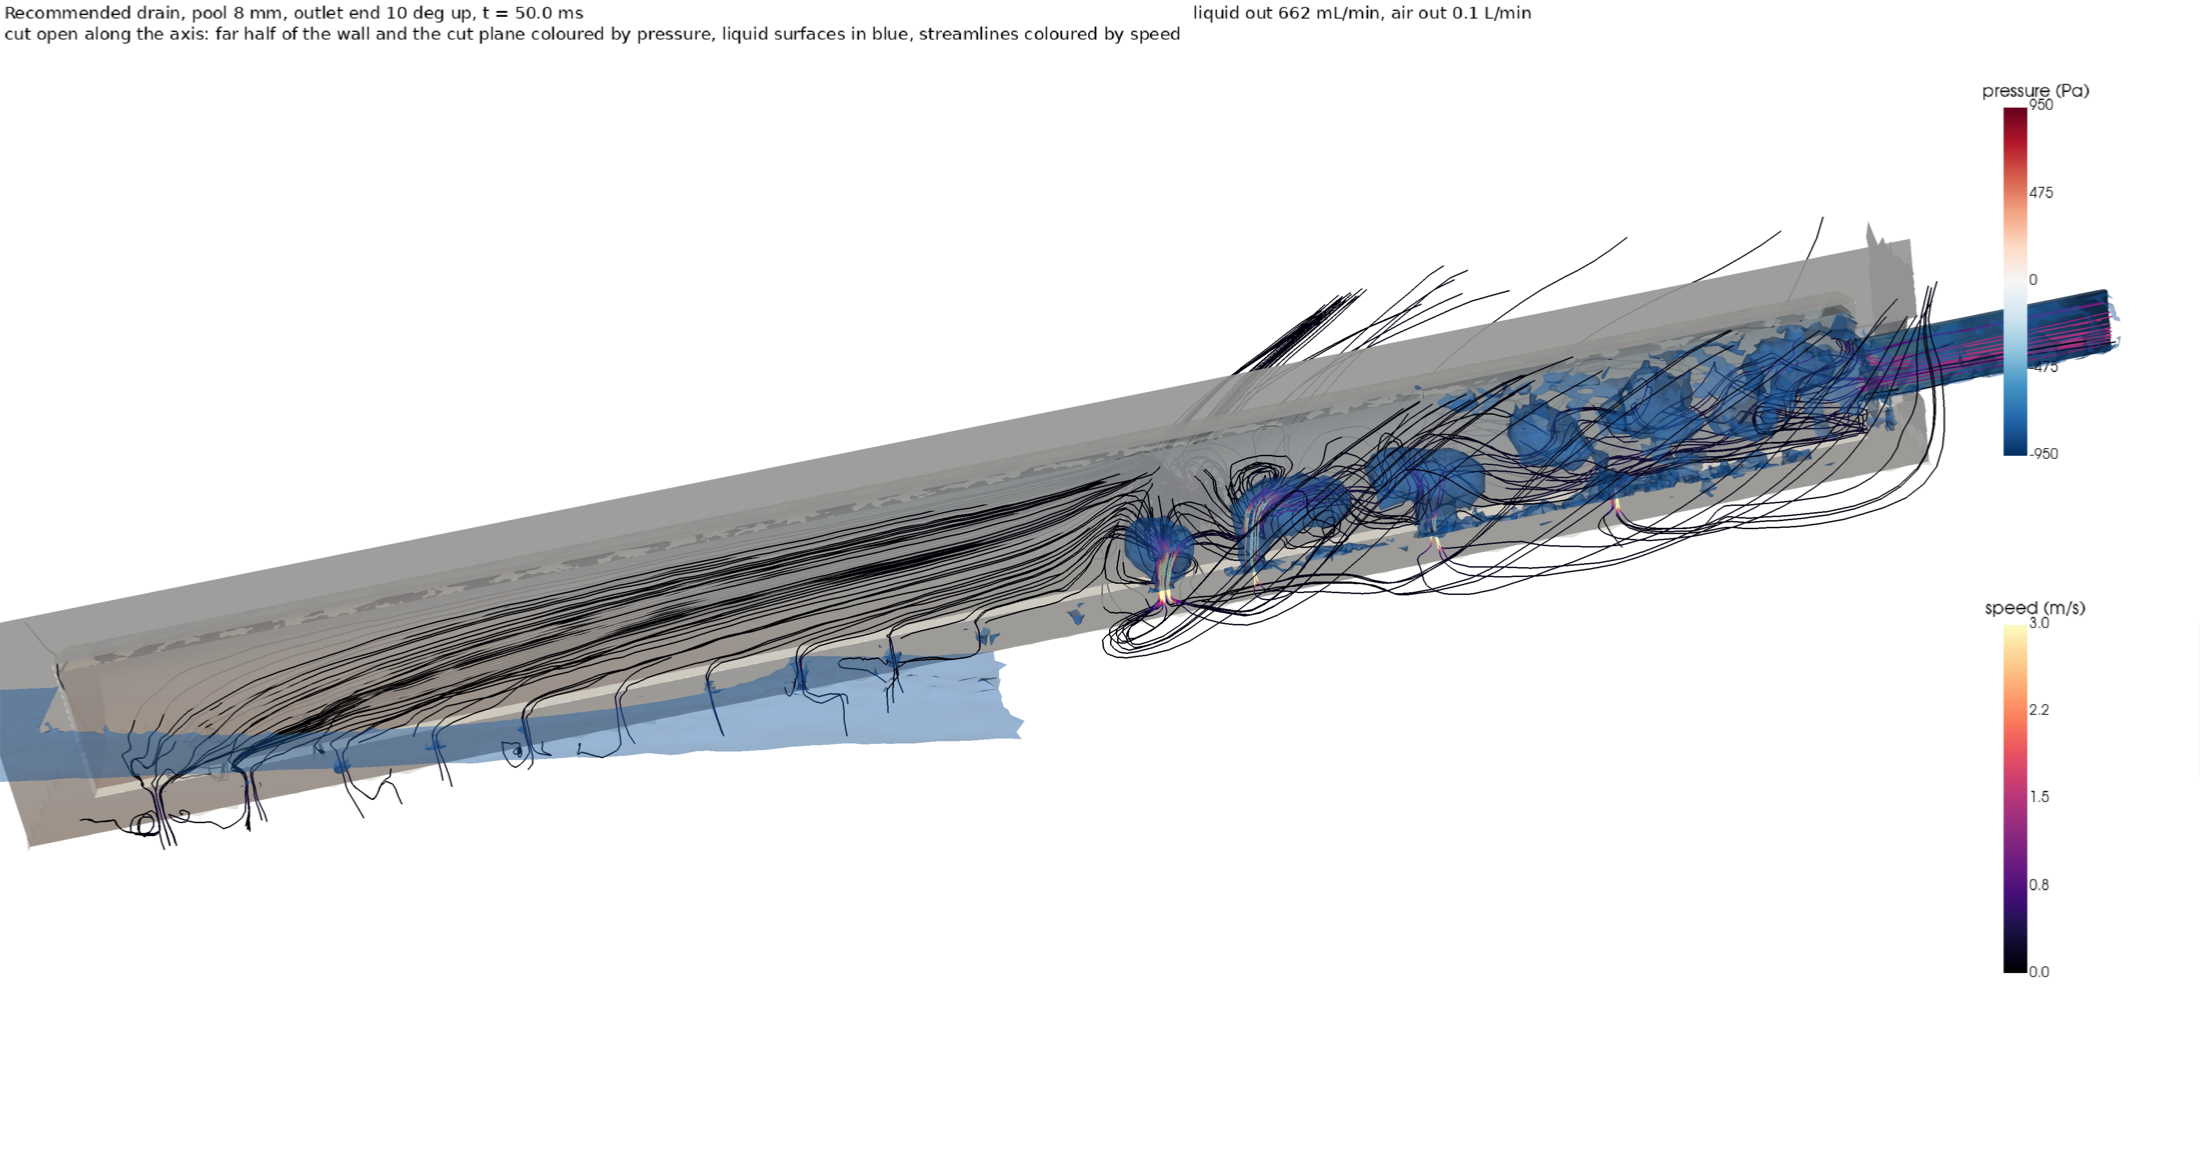
\includegraphics[width=\linewidth]{cfd_rec_cut3d.png}\\[2mm]
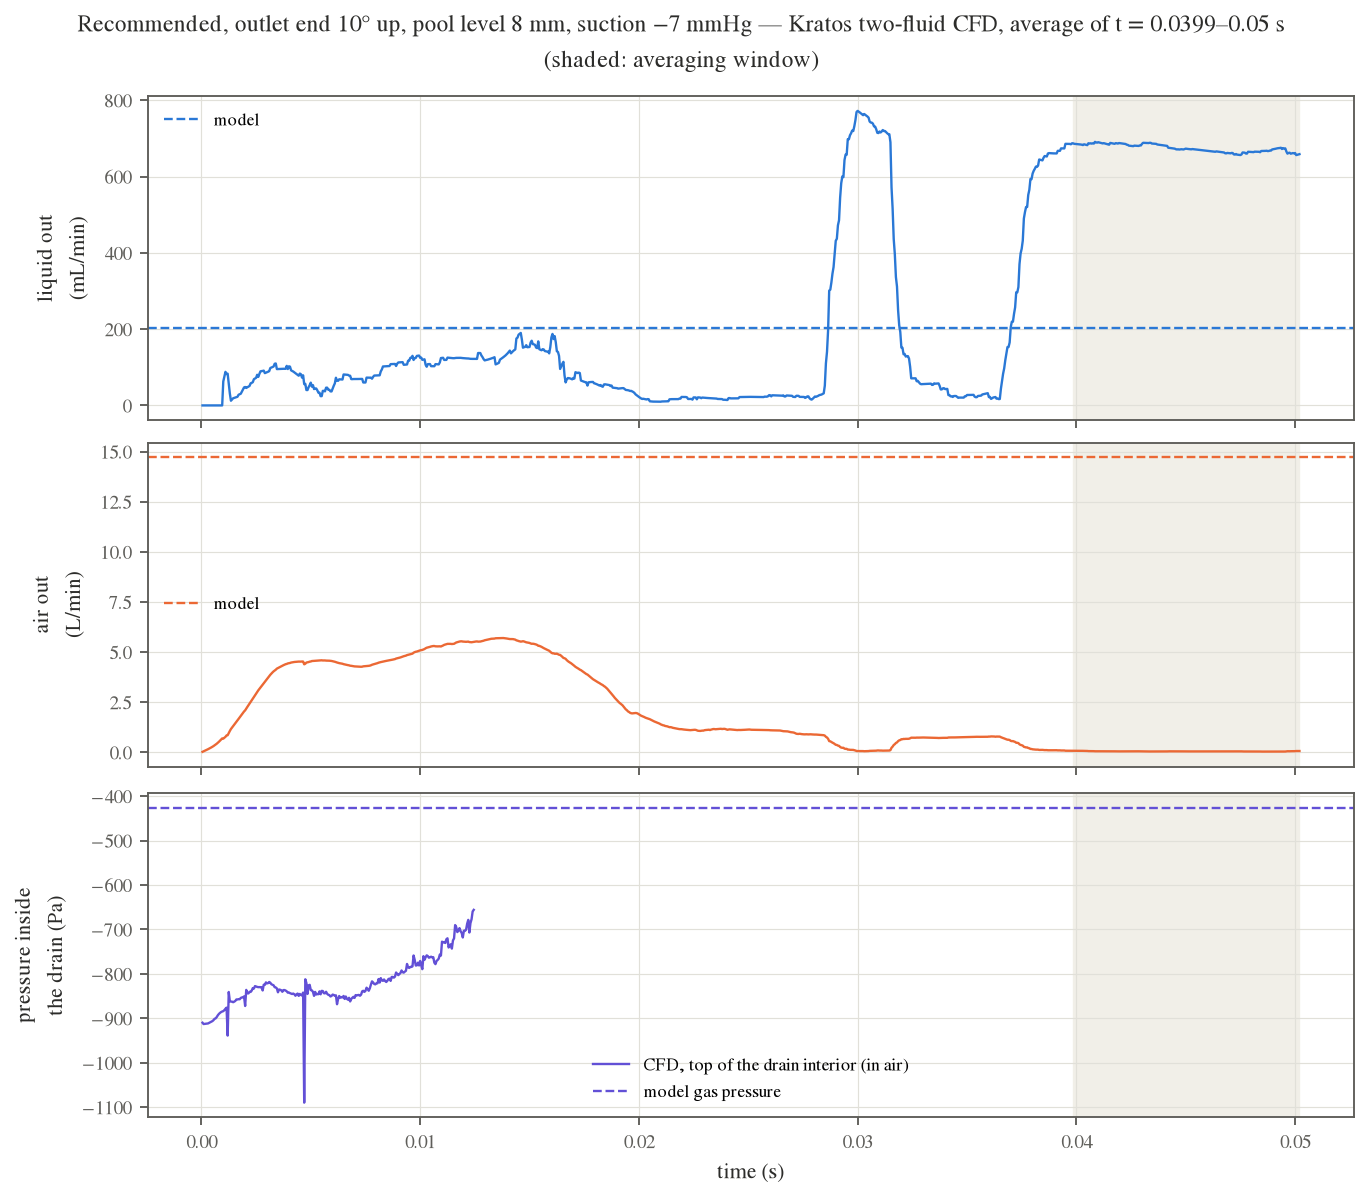
\includegraphics[width=0.8\linewidth]{cfd_rec_history.png}
\caption{Recommended layout, pool at 8\,mm. Top: the drain at 50\,ms, cut open along its axis. The far half of the wall and the cut plane are coloured by pressure, liquid surfaces and air bubbles are blue, and streamlines are coloured by speed. Bottom: the liquid and air flow at the outlet and the air pressure at the top of the interior against time, with the model's values dashed. After 12\,ms no probe at the top of the interior is in air, so the pressure curve ends.}
\label{fig:cfd-rec}
\end{figure}

\paragraph{What the CFD shows, and what it does not.}
\begin{itemize}
\item \textbf{It confirms the mechanism the model is built on.} Exposed openings draw air at $-7$\,mmHg. That air flows along the top of the interior into the bore and uses up most of the bore's capacity.
\item \textbf{It agrees with the model near the as-built drain's stop.} With the as-built field at 21\,mm, the outlet carries mainly air and little liquid, as the model predicts 1\,mm above its stop level. The air flow agrees within 30\,\%.
\item \textbf{It does not confirm the stop levels quantitatively.} The runs are short (15 and 50\,ms) and the recommended case is still in its start-up. The openings have only 3--4 cells across, surface tension is not modelled, and the trough is small. The stop levels therefore still rest on the two reduced-order simulations of Section~\ref{sec:sim}.
\end{itemize}

% =============================================================================
\section{Limitations}\label{sec:limits}
\begin{itemize}
\item \textbf{Model order.} The model is a reduced-order network, not a 3D volume-of-fluid simulation. Slug and churn flow in the bore, foaming, and unsteady sloshing are represented only by the separated-phase bore model.
\item \textbf{Interior.} The interior is one open lumen; the flow distribution along it (a suction manifold~\cite{bajura1976}) matters only for flow rates. The fluted inner wall and core of the as-built part add axial resistance, which changes flow rates and drain times but not the stop levels, since no liquid flows at the stop.
\item \textbf{Hole and bore laws.} The discharge coefficients and the additive Sampson--Poiseuille law are standard correlations, not fitted to this part. The stop level is insensitive to them (Table~\ref{tab:sens}).
\item \textbf{Capillarity and drawdown.} These are treated with simple bounds. The real contact angle of the drain material should be measured.
\item \textbf{Tissue and clots.} Tissue contact and clotting are outside the model; the existing FEBio work in the project addresses tissue sealing a hole.
\item \textbf{CFD check is qualitative.} The 3D two-phase runs of Section~\ref{sec:cfd} confirm the air-leak mechanism and the near-stop state of the as-built drain, but they are short and coarse at the openings. The stop levels are confirmed quantitatively only by the two reduced-order simulations.
\end{itemize}

% =============================================================================
\section{Conclusions}
\begin{enumerate}
\item \textbf{Exposed holes always leak.} At $-7$\,mmHg ($H_v=\numHv$\,mm), every hole of 0.5 to 4\,mm lets air in once it is exposed; capillary sealing would need holes below \numdstar\,mm.
\item \textbf{The stop condition.} The air leak and the outlet bore form a pressure divider. Drainage stops when $h+H_v/(1+\Lw^2)=\zl$, or when no hole is left below the surface. Two independent simulations confirm this.
\item \textbf{Tilt is the critical case.} When the drain lies flat, every layout drains to just below the bore lip (2.7\,mm). With the outlet up, the lip rises by $L\sin\alpha$, and only a small exposed-area ratio keeps the vacuum high enough to lift the liquid there.
\item \textbf{What decides the result.} Hole size matters only through the total open area and the coverage of the length. Too much area (as built: 468\,mm$^2$) stops the drain at 20\,mm with the outlet $10^\circ$ up; too few, large holes leave the ends uncovered.
\item \textbf{Recommendation.} Use two staggered rows at $\pm30^\circ$ with $36\times$\O1.0\,mm (2 times the bore area). This drains to the lowest hole edge from $-10^\circ$ to $+22^\circ$ while keeping 81\,\% of the maximum flow. With the intended wall regulator this needs at least \numcapTwenty\,L/min of air flow at $-7$\,mmHg; with a weaker source, use fewer holes (Table~\ref{tab:pump}).
\end{enumerate}

\sloppy
\paragraph{Reproduction.} All code is in \texttt{drain/drainstop}: \texttt{drainstop/model.py} (geometry, hydraulics, network solver, closed form), \texttt{drainstop/transient.py} (time-dependent model), \texttt{scripts/run\_study.py} (all studies, $\sim$10\,min on 12 cores), \texttt{scripts/make\_figures.py}, \texttt{scripts/make\_tables.py} and \texttt{scripts/make\_pictures.py} (Fig.~\ref{fig:pictures}); the 3D CFD (Kratos, Windows) and its results are in \texttt{vof/kratos/}; an OpenFOAM set-up is in \texttt{vof/} (Euler) and \texttt{vof/local/} (Linux).

\begin{thebibliography}{99}\small
\bibitem{sampson1891} R.~A. Sampson, On Stokes's current function, \emph{Phil. Trans. R. Soc. Lond. A} 182 (1891) 449--518.
\bibitem{dagan1982} Z. Dagan, S. Weinbaum, R. Pfeffer, An infinite-series solution for the creeping motion through an orifice of finite length, \emph{J. Fluid Mech.} 115 (1982) 505--523.
\bibitem{lichtarowicz1965} A. Lichtarowicz, R.~K. Duggins, E. Markland, Discharge coefficients for incompressible non-cavitating flow through long orifices, \emph{J. Mech. Eng. Sci.} 7 (1965) 210--219.
\bibitem{idelchik1994} I.~E. Idelchik, \emph{Handbook of Hydraulic Resistance}, 3rd ed., Begell House, 1994.
\bibitem{oliver1977} J.~F. Oliver, C. Huh, S.~G. Mason, Resistance to spreading of liquids by sharp edges, \emph{J. Colloid Interface Sci.} 59 (1977) 568--581.
\bibitem{degennes2004} P.-G. de Gennes, F. Brochard-Wyart, D. Qu\'er\'e, \emph{Capillarity and Wetting Phenomena}, Springer, 2004.
\bibitem{cheng2008} N.-S. Cheng, Formula for the viscosity of a glycerol--water mixture, \emph{Ind. Eng. Chem. Res.} 47 (2008) 3285--3288.
\bibitem{wallis1969} G.~B. Wallis, \emph{One-Dimensional Two-Phase Flow}, McGraw-Hill, 1969.
\bibitem{gordon1970} J.~L. Gordon, Vortices at intakes, \emph{Water Power} 22 (1970) 137--138.
\bibitem{bajura1976} R.~A. Bajura, E.~H. Jones, Flow distribution manifolds, \emph{J. Fluids Eng.} 98 (1976) 654--665.
\end{thebibliography}

\end{document}
